\batchmode
\makeatletter
\def\input@path{{"C:/Users/tkpme/Dropbox/BookPCRA/Springer Production March 2026/Ch Appendix E Machine Learning/"}}
\makeatother
\documentclass[graybox,envcountchap,sectrefs]{svmono}\usepackage[]{graphicx}\usepackage[]{xcolor}
% maxwidth is the original width if it is less than linewidth
% otherwise use linewidth (to make sure the graphics do not exceed the margin)
\makeatletter
\def\maxwidth{ %
  \ifdim\Gin@nat@width>\linewidth
    \linewidth
  \else
    \Gin@nat@width
  \fi
}
\makeatother

\definecolor{fgcolor}{rgb}{0.345, 0.345, 0.345}
\newcommand{\hlnum}[1]{\textcolor[rgb]{0.686,0.059,0.569}{#1}}%
\newcommand{\hlsng}[1]{\textcolor[rgb]{0.192,0.494,0.8}{#1}}%
\newcommand{\hlcom}[1]{\textcolor[rgb]{0.678,0.584,0.686}{\textit{#1}}}%
\newcommand{\hlopt}[1]{\textcolor[rgb]{0,0,0}{#1}}%
\newcommand{\hldef}[1]{\textcolor[rgb]{0.345,0.345,0.345}{#1}}%
\newcommand{\hlkwa}[1]{\textcolor[rgb]{0.161,0.373,0.58}{\textbf{#1}}}%
\newcommand{\hlkwb}[1]{\textcolor[rgb]{0.69,0.353,0.396}{#1}}%
\newcommand{\hlkwc}[1]{\textcolor[rgb]{0.333,0.667,0.333}{#1}}%
\newcommand{\hlkwd}[1]{\textcolor[rgb]{0.737,0.353,0.396}{\textbf{#1}}}%
\let\hlipl\hlkwb

\usepackage{framed}
\makeatletter
\newenvironment{kframe}{%
 \def\at@end@of@kframe{}%
 \ifinner\ifhmode%
  \def\at@end@of@kframe{\end{minipage}}%
  \begin{minipage}{\columnwidth}%
 \fi\fi%
 \def\FrameCommand##1{\hskip\@totalleftmargin \hskip-\fboxsep
 \colorbox{shadecolor}{##1}\hskip-\fboxsep
     % There is no \\@totalrightmargin, so:
     \hskip-\linewidth \hskip-\@totalleftmargin \hskip\columnwidth}%
 \MakeFramed {\advance\hsize-\width
   \@totalleftmargin\z@ \linewidth\hsize
   \@setminipage}}%
 {\par\unskip\endMakeFramed%
 \at@end@of@kframe}
\makeatother

\definecolor{shadecolor}{rgb}{.97, .97, .97}
\definecolor{messagecolor}{rgb}{0, 0, 0}
\definecolor{warningcolor}{rgb}{1, 0, 1}
\definecolor{errorcolor}{rgb}{1, 0, 0}
\newenvironment{knitrout}{}{} % an empty environment to be redefined in TeX

\usepackage{alltt}
\usepackage{mathptmx}
\usepackage{helvet}
\usepackage{courier}
\usepackage[T1]{fontenc}
\usepackage[utf8]{inputenc}
\usepackage{geometry}
\geometry{verbose,tmargin=1in,bmargin=1in,lmargin=1in,rmargin=1in}
\setcounter{tocdepth}{3}
\setlength{\parskip}{\medskipamount}
\setlength{\parindent}{0pt}
\usepackage{float}
\usepackage{booktabs}
\usepackage{units}
\usepackage{textcomp}
\usepackage{mathrsfs}
\usepackage{url}
\usepackage{amsmath}
\usepackage{amssymb}
\usepackage{graphicx}
\PassOptionsToPackage{normalem}{ulem}
\usepackage{ulem}
\usepackage[unicode=true,pdfusetitle,
 bookmarks=true,bookmarksnumbered=true,bookmarksopen=true,bookmarksopenlevel=1,
 breaklinks=false,pdfborder={0 0 1},backref=false,colorlinks=false]
 {hyperref}
\hypersetup{
 pdfstartview=XYZ null null 1.25,pdfpagemode=UseNone}

\makeatletter

%%%%%%%%%%%%%%%%%%%%%%%%%%%%%% LyX specific LaTeX commands.
%% Because html converters don't know tabularnewline
\providecommand{\tabularnewline}{\\}
\floatstyle{ruled}
\newfloat{algorithm}{tbp}{loa}[chapter]
\providecommand{\algorithmname}{Algorithm}
\floatname{algorithm}{\protect\algorithmname}

%%%%%%%%%%%%%%%%%%%%%%%%%%%%%% User specified LaTeX commands.
%%%%%%%%%%%%%%%%%%%% book.tex %%%%%%%%%%%%%%%%%%%%%%%%%%%%%
%
% sample root file for the chapters of your "monograph"
%
% Use this file as a template for your own input.
%
%%%%%%%%%%%%%%%% Springer-Verlag %%%%%%%%%%%%%%%%%%%%%%%%%%


% RECOMMENDED %%%%%%%%%%%%%%%%%%%%%%%%%%%%%%%%%%%%%%%%%%%%%%%%%%%


% choose options for [] as required from the list
% in the Reference Guide

\usepackage{makeidx}% allows index generation
% standard LaTeX graphics tool
                             % when including figure files
\usepackage{multicol}% used for the two-column index
\usepackage[bottom]{footmisc}% places footnotes at page bottom

\usepackage{hyperref}
\def\UrlBreaks{\do\/\do-}

% see the list of further useful packages
% in the Reference Guide

\makeindex             % used for the subject index
                       % please use the style svind.ist with
                       % your makeindex program


%\usepackage[ style=authoryear,natbib=true,giveninits=true,backend=biber,maxcitenames=2]{biblatex}
\usepackage[style=authoryear,natbib=true,firstinits=false,backend=biber,maxcitenames=2]{biblatex}


\setlength{\bibitemsep}{0.5\baselineskip}
\DeclareNameAlias{sortname}{family-given}

\IfFileExists{C:/Users/Doug/Dropbox/BookPCRA/mpslbookCombined.bib}
{\addbibresource[location=local]{C:/Users/Doug/Dropbox/BookPCRA/mpslbookCombined.bib}}
{   \IfFileExists{C:/Users/tkpme/Dropbox/BookPCRA/mpslbookCombined.bib}
    {\addbibresource[location=local]{C:/Users/tkpme/Dropbox/BookPCRA/mpslbookCombined.bib}}
    {   \IfFileExists{C:/Users/stoya/Dropbox/BookPCRA/mpslbookCombined.bib}
        {\addbibresource[location=local]{C:/Users/stoya/Dropbox/BookPCRA/mpslbookCombined.bib}}
        {   \IfFileExists{C:/Users/4thauthor/Dropbox/BookPCRA/mpslbookCombined.bib}
            {\addbibresource[location=local]{C:/Users/4thauthor/Dropbox/BookPCRA/mpslbookCombined.bib}}
            {}
        }
    }
}
\renewcommand\cite{\citet}

\usepackage{amsmath}
\usepackage{amssymb}
\usepackage[p,osf]{stickstootext}
\usepackage[stix2,vvarbb]{newtxmath}
\usepackage[varqu,varl]{inconsolata}
% \usepackage{txfonts}
\usepackage{upgreek}

\DeclareMathOperator{\argmax}{arg\,max}
\DeclareMathOperator{\argmin}{arg\,min}
\usepackage{array}
\usepackage{arydshln}
\usepackage{booktabs}
\usepackage{threeparttablex}
\usepackage{appendix}

\usepackage[utf8]{inputenc}
%%%%%%%%%%%%%%%%%%%%%%%%%%%%%%%%%%%%%%%%%%%
\IfFileExists{C:/Users/Doug/Dropbox/BookPCRA/macroSP_August_05_2021.tex}
{\input{C:/Users/Doug/Dropbox/BookPCRA/macroSP_August_05_2021.tex}}
{   \IfFileExists{C:/Users/tkpme/Dropbox/BookPCRA/macroSP_August_05_2021.tex}
    {\input{C:/Users/tkpme/Dropbox/BookPCRA/macroSP_August_05_2021.tex}}
    {   \IfFileExists{C:/Users/stoya/Dropbox/BookPCRA/macroSP_August_05_2021.tex}
        {\input{C:/Users/stoya/Dropbox/BookPCRA/macroSP_August_05_2021.tex}}
        {   \IfFileExists{C:/Users/4thAuthor/Dropbox/BookPCRA/macroSP_August_05_2021.tex}
            {\input{C:/Users/4thAuthor/Dropbox/BookPCRA/macroSP_August_05_2021.tex}}
            {}
        }
    }
}

\belowsink=90pt

%%%%%%%%%%%%%%%%%%%%%%%%%%%%%%%%%%%%%%%%%%%%%

\makeatother
\IfFileExists{upquote.sty}{\usepackage{upquote}}{}
\begin{document}
\begin{appendices}


\setcounter{chapter}{4} 

\chapter{MACHINE LEARNING\label{chap:AppendixE}}

\vspace{0.3in}

\textbf{Planned for publication in 2026 by R. Douglas Martin, Thomas
K. Philips, Bernd Scherer and Kirk Li. All rights reserved. © Copyright
2025}

\vspace{0.3in}

\begin{center}
10/22/25
\par\end{center}

\tocchpnum=30pt 
\tocsecnum=33pt 
\tocsubsecnum=40pt 
\tocsubsubsecnum=48pt 
\tocparanum=55pt 
\tocsubparanum=63pt
\calctocindent

\tableofcontents{}\newpage{}

\section{Overview of Machine Learning }

Machine Learning (ML), Large Language Models (LLMs), and Generative
Artificial Intelligence (GAI) have had a significant impact on a variety
of fields, and we fully expect portfolio management to prove no less
vulnerable to their disruptive effects. \citet{Breiman2001} identifies
two disjoint statistical cultures:
\begin{enumerate}
\item A data--driven culture that is focused on modeling data as if it
were drawn from a known data model, which is universally assumed to
be a parametric distribution whose parameters can be estimated, ideally
by maximum-likelihood, and fitting system responses (or dependent
variables) to data items (or independent variables) using methods
appropriate to the distribution (e.g. linear regression /least squares
for jointly normal random variables), with goodness-of-fit being the
primary figure of merit, and
\item A distribution--agnostic culture that is focused on identifying an
(often high-dimensional) algorithmic relationship between the data
and the system's responses, with forecast accuracy being the primary
figure of merit. 
\end{enumerate}
\citet{Breiman2001} argues that while most statisticians fall into
the first group, it is the second group that is focused on what truly
matters in the real world, and we might call members of the second
group ML practitioners. Loosely speaking, ML refers to 
\begin{enumerate}
\item Novel application of statistical and algorithmic methods and non-linear
transformations to high-dimensional data,\footnote{See for example, the material on identifying recesssions and recoveries
in \ExpectedReturnChapter, where the raw unemployment rate must be
transformed before it can be input to a threshold detector.} as well as the use of non-linear models (e.g. multiplicative models,
or models with interaction terms) in order to solve numerical problems
such as forecasting future stock returns from current prices and financial
statement information, and
\item Automatic model selection using regularized regression, as well as
by applying measures of model complexity such as AIC (\citet{Akaike1974})
and BIC (\citet{Schwarz1978}, as well as \citet{deLeeuw1992}), and
of predictive power, such as the Robust Final Predictor Error method
covered in \TimeSeriesFactorModelsChapter. This type of machine learning
has been in use for over fifty years, and continues to be developed
with new techniques for model selection even when the data sets are
not huge, and when the number of variables used is modest. 
\end{enumerate}
LLMs and GAI, on the other hand, first transform, and then process,
textual or visual data to solve unstructured problems such as summarizing
news items, regulatory testimony, or management disclosures in corporate
financial statements. ML, LLMs, and GAI should not be seen as mutually
exclusive fields. They are better thought of as existing along a continuum,
as the techniques and algorithms that underpin them have much in common. 

\citet{KellyXiu2023} comprehensively survey the application of Machine
Learning methods to problems in finance, and \citet{HastieTibshiraniFriedman2009}
and \citet{JWHTStatLearning2013} provide rigorous, insightful, and
thoughtful coverage of the statistical aspects of machine learning.
\citet{GuKellyXiu2020} and \citet{CaoJiangWangYang2024} exemplify
the application of these methods to asset pricing and the estimation
of expected returns, while \citet{KimMuhnNikolaev2023}, \citet{KimMuhnNikolaev2024a}
and \citet{KimMuhnNikolaev2024b} exemplify the application of Large
Language Models and Generative Artificial Intelligence to the comprehension
of financial statements.

The distinguishing features of machine learning methods are their
ability to efficiently handle exceptionally large data sets with many
explanatory factors, their focus on model selection and mitigating
overfits to noisy data, and their ability to model the non-linearities
that characterize most real-world problems.

A thoughtful investor must embrace both financial and technological
perspectives when employing ML, LLMs, and GAI -- the risk of lazy
inquiry is the identification of models devoid of economic underpinnings
that are modern day equivalents of constellations in a night sky studded
with stars. The all-too-common consequence of such practices is models
that generate good results when tested with available data, but which
fail miserably when faced with new data. It is fair to say that the
field of machine learning has grown so explosively in recent years
that a portion of an appendix cannot do it justice, and we therefore
focus on a small, but important, subset of such methods that are of
particular relevance to portfolio management.

Machine Learning algorithms can usefully be classified into three
categories:
\begin{enumerate}
\item Supervised learning: An algorithm is presented with a set of inputs
or \emph{features} (e.g. financial statements and market data) and
outputs or \emph{responses} (e.g. stock market returns) and is tasked
with identifying the relationship between the two. Formally, given
a collection of feature--response pairs $\left[\mathbf{X},\ \mathbf{y}\right]=\left\{ \mathbf{x}_{i},\ \mathbf{y}_{i}\right\} ,\ 1\leqslant i\leqslant N$,
as well as a corresponding set of (usually non--negative) weights
$w_{i}$ and a loss function $\mathscr{L}$, find a high--dimensional
function $f$ such that $\sum_{i}w_{i}\,\mathscr{L}\left(f\left(\mathbf{x}_{i}\right)-\mathbf{y}_{i}\right)$
is minimized. It is often assumed, frequently without justification,
that the features and the responses are linearly related to each other,
and it good practice to explore the creation of new features by applying
non-linear transformations to existing features. 
\item Unsupervised learning: An algorithm is presented with a collection
of objects (e.g., bonds), each with a set of characteristics (e.g.,
covenants, spreads, issuer's financial statements and history of defaults)
and is tasked with estimating the high--dimensional joint density
of the data, or of classifying it into a set of disjoint clusters
such that the items in each cluster are close to each other under
some metric, and are distant from items in other clusters. In the
given example, the clusters might be ratings classes. 
\item Reinforcement learning: An algorithm is presented with an initial
set of inputs and an objective function which it is tasked with maximizing.
New inputs are continually incorporated and consumed, and an optimal
response is recomputed following each new observation. In this case,
the reinforcement learning algorithm may be thought of as an optimal
control policy, and can be applied to the multi-period optimization
of a portfolio whose holdings have time-varying expected returns and
transaction costs.
\end{enumerate}

We restrict our exploration of machine learning to the field of \emph{supervised
learning} -- a form of learning that is particularly relevant to
portfolio management, and Least Squares and its variants prove to
be a good starting point for many supervised learning algorithms,
as does exploratory data analysis (EDA). The R packages \texttt{tourr}
and \texttt{Pursuit} are particularly useful for EDA as they allow
users to explore and visualize large multivariate datasets, project
the data along different axes, and to tour the projections to identify
clusters visually.


\section{Supervised Learning Using Regularized Classical Algorithms\label{sec:ClassicalSupervisedLearning}}

The classical linear model\footnote{We include the sizes of the various vectors and matrices as subscripts
for clarity.}

\begin{equation}
\mathrm{\mathbf{y}}_{N\times1}=\mathrm{\mathbf{X}}_{N\times p}\ \bubeta_{N\times1}\,+\,\bueps_{N\times1}\label{eq:OLS1}
\end{equation}

which is used for time series and cross-section factor models in \FactorModelsChapters,
and is described in detail in \ProbabilityAppendix\ minimizes $\bueps_{1\times N}^{\prime}\ \bueps_{N\times1}$
and is given by

\begin{align}
\hat{\bubeta}_{LS} & =\underset{\bubeta}{\mathrm{argmin}}\ \bueps_{1\times N}^{\prime}\ \bueps_{N\times1}\nonumber \\
 & =\left(\mathrm{\mathbf{X}}_{p\times N}^{\prime}\ \mathrm{\mathbf{X}}_{N\times p}\right)^{-1}\ \mathrm{\mathbf{X}}_{p\times N}^{\prime}\ \mathrm{\mathbf{y}}_{N\times1}.\label{eq:OLS2}
\end{align}

 

Equation \eqref{eq:OLS2} gives us insights into the limitations of
Least Squares and its region of applicability.
\begin{enumerate}
\item If $p>N$, no unique solution exists because $\mathrm{\mathbf{X}}_{p\times N}^{\prime}\,\mathrm{\mathbf{X}}_{N\times p}$
is singular. None the less, this is an important use case in genomics
(see \citet{JohnstoneTitterington2009} and \citet{FanMaZhong2021})
and is increasingly important in finance, as researchers often throw
every explanatory variable they have available into ``kitchen sink''
regressions in the hope of identifying a factor relevant to the problem
at hand. This issue is addressed in depth in \ExpectedReturnChapter.
\item If the columns of $\mathbf{X}$ are nearly co-linear because some
of the explanatory variables are closely related to, or constructed
in almost the same way as others (e.g. Comprehensive Income, Net Income
and Operating Income, all from the Income Statement of a firm's financial
statements), $\mathrm{\mathbf{X}}_{p\times N}^{\prime}\,\mathrm{\mathbf{X}}_{N\times p}$
becomes nearly singular, and the coefficient estimates become unstable.
\item Least squares does not perform variable selection: even if the true
relationship between $\mathrm{\mathbf{X}}$ and $\mathrm{\mathbf{y}}$
is encapsulated in a small subset of the entries in $\mathrm{\bubeta}$,
Least Squares will likely assign non-zero values to all its entries. 
\item If the true relationship between $\mathrm{\mathbf{X}}$ and $\mathrm{\mathbf{y}}$
is non-linear, any transformation of the columns of $\mathrm{\mathbf{X}}$
needs to be done ahead of time by the analyst. This, too, is addressed
in \ExpectedReturnChapter, where it is shown that the addition of
a quadratic term noticeably improves return forecasts for the S\&P
500.
\item Least Squares is not robust to even a single outlier, and we refer
the reader to \RobustEstimationSections, where robust methods are
introduced as data dependent weighted versions of least squares estimators,
as well as to \RobustEstimatorsChapter, whichdescribes robust regression
algorithms that are largely unaffected by outliers, and which should
be used routinely by financial analysts.
\end{enumerate}
Some, though not all, of these problems can be addressed using \emph{regularization}
techniques which are designed to reduce the likelihood of overfitting
models to data, and which we next discuss.


\subsection{Regularization}

The central idea that underlies regularization is simple: constrain
the weights $\bubeta$ in some way so that they become more stable
and/or more sparse, and computable even if $p>N$. For notational
simplicity, we assume that all the columns of $\mathrm{\mathbf{X}}$
as well as $\mathrm{\mathbf{y}}$ are demeaned, so that the first
element of $\bubeta$ corresponds to an explanatory variable, and
not the intercept. This is standard practice when regularizing --
it is variations from a baseline, not the baseline itself, that we
are trying to fit, and shrinking the intercept will immediately introduce
bias. Define

\begin{align}
\left\Vert \bueps\right\Vert ^{2} & =\bueps^{\prime}\bueps.\nonumber \\
 & =\left(\mathrm{\mathbf{y}}\,-\,\mathrm{\mathbf{X}}\,\bubeta\right)^{\prime}\left(\mathrm{\mathbf{y}}\,-\,\mathrm{\mathbf{X}}\,\bubeta\right)\label{eq:SumEpsilonSquared}
\end{align}

and

\begin{equation}
\left\Vert \bubeta\right\Vert _{q}=\sum_{i\,=\,1}^{p}\left|\bubeta_{i}\right|^{q},\ \ q\geqslant0.\label{eq:qNormBeta}
\end{equation}

While it is common practice to write$\left\Vert \mathbf{x}\right\Vert _{q}=\left(\sum_{i\,=\,1}^{p}\left|\mathbf{x}_{i}\right|^{q}\right)^{1/q}$,
we have deliberately chosen not to raise the sum in \eqref{eq:qNormBeta}
to the $1/q^{th}$ power as $q=0$ is an important special case --
$\left\Vert \bubeta\right\Vert _{0}$ is just the number of non-zero
components of $\bubeta$.\footnote{It is standard practice in this context to assume that $0^{0}=0$.}
When $q=1$, it is the sum of their absolute values, and when $q=2$,
it is the square of the Euclidean length of $\bubeta$. Regularization
reformulates the least squares objective function to

\begin{equation}
\hat{\bubeta}_{q}=\underset{\bubeta}{\mathrm{argmin}}\ \left\Vert \bueps\right\Vert ^{2}\,+\,\lambda_{q}\left\Vert \bubeta\right\Vert _{q},\ \ q,\ \lambda_{q}\geqslant0\label{eq:RegularizationGeneral}
\end{equation}

When $\lambda_{q}=0$, we are back to classical Least Squares for
all $q\geqslant0$. When $q=0$ and $\lambda_{0}>0$, we are trading
off Mean Squared Error against the number of predictor variables.
When $q=1$ and $\lambda_{1}>0$ , we are trading off Mean Squared
Error against the sum of the magnitude of all the coefficients. This
case is known as \emph{lasso} (\uline{L}east \uline{A}bsolute
\uline{S}hrinkage and \uline{S}election \uline{O}perator,
\citet{Tibshirani1996}, \citet{Tibshirani2011}). When $q=2$ and
$\lambda_{2}>0$, we are trading off Mean Squared Error against the
square of the Euclidean length of the coefficient vector. This case
is known as \emph{ridge regression} (\citet{HoerlKennard1970}, \citet{Hastie2020}).\footnote{Technometrics devoted an entire issue (Vol 62, Issue 4, 2020) to celebrate
the $50^{th}$ anniversary of ridge regression.} The optimal value of $\lambda$ is determined using \emph{cross-validation},
which we discuss below. 

Figure \ref{fig:ContraintSurfaces} illustrates the shape of the constraint
boundaries for lasso, ridge regression, and the elastic net, which
is a weighted linear combination of the lasso and ridge penalties,
with two explanatory variables. All three boundaries are convex, but
only the latter two are strictly convex. The \texttt{R} package \texttt{glmnet}
(\url{https://glmnet.stanford.edu/index.html}) provides efficient
implementations of all these methods as well as many others. 

\begin{figure}[H]
\begin{centering}
\includegraphics[scale=0.7]{5C__Users_tkpme_Dropbox_BookPCRA_Springer_Produ___ots_Lasso_Ridge_and_Elastic_Net_Constraints.png}
\par\end{centering}
\caption{\label{fig:ContraintSurfaces}Shape of the Contraint Surfaces for
Lasso, Ridge and Elastic Net For Two Variables}
\end{figure}


\subsection{Ridge Regression}

The objective function for ridge regression can be written in two
equivalent ways:

\begin{subequations}
\begin{align}
\hat{\bubeta}_{ridge} & =\underset{\bubeta}{\mathrm{argmin}}\ \left\Vert \bueps\right\Vert ^{2}\,+\,\lambda\left\Vert \bubeta\right\Vert _{2},\ \ \lambda>0\label{eq:RidgeRegressionA}\\
 & =\underset{\bubeta}{\mathrm{argmin}}\ \left\Vert \bueps\right\Vert ^{2},\ \ \mathrm{s.t.}\left\Vert \bubeta\right\Vert _{2}\leqslant c,\ c>0\label{eq:RidgeRegressionB}
\end{align}
\end{subequations}

These formulations echo the two ways in which efficient frontiers
can be computed (the Lagrangian formulation and the bound formulation),
but the Lagrangian formulation \eqref{eq:RidgeRegressionA} is easier
to deal with analytically. The bound formulation makes clear that
$\bubeta$ lies on or inside the surface of a hypersphere of radius
$\sqrt{c}.$ In fact, it mirrors the formulation of mean-variance
efficient portfolio construction covered in \FoundationsChapter. 

Ridge regression was originally proposed by \citet{HoerlKennard1970}
as an ad-hoc solution to the problem of collinearity in least squares.
It is sometimes said to get its name from the fact that it adds a
stabilizing ``raised ridge'' to the diagonal of $\mathrm{\mathbf{X}}^{\prime}\ \mathrm{\mathbf{X}}$.
The quadratic penalty term ensures that closed form solutions to \eqref{eq:RidgeRegressionA}
and \eqref{eq:RidgeRegressionB} always exists, and it is left as
an exercise to show that 

\begin{equation}
\hat{\bubeta}_{ridge}=\left(\mathrm{\mathbf{X}}_{p\times N}^{\prime}\,\mathrm{\mathbf{X}}_{N\times p}\,+\,\lambda\,\mathbf{I}_{p\times p}\right)^{-1}\,\mathrm{\mathbf{X}}_{p\times N}^{\prime}\,\mathrm{\mathbf{y}}_{N\times1},\label{eq:RidgeRegressionSolution}
\end{equation}

that the $p$ eigenvalues of $\mathrm{\mathbf{X}}_{p\times N}^{\prime}\,\mathrm{\mathbf{X}}_{N\times p}\,+\,\lambda\,\mathbf{I}_{p\times p}$
can be obtained by adding $\lambda$ to the eigenvalues of $\mathrm{\mathbf{X}}_{p\times N}^{\prime}\,\mathrm{\mathbf{X}}_{N\times p}$,
and that the eigenvectors of $\mathrm{\mathbf{X}}_{p\times N}^{\prime}\,\mathrm{\mathbf{X}}_{N\times p}\,+\,\lambda\,\mathbf{I}_{p\times p}$
are identical to the eigenvectors of $\mathrm{\mathbf{X}}_{p\times N}^{\prime}\,\mathrm{\mathbf{X}}_{N\times p}$.
Simple rearrangement of \eqref{eq:OLS2} and \eqref{eq:RidgeRegressionSolution}
shows that

\begin{equation}
\hat{\bubeta}_{ridge}=\left(\mathbf{I}_{p\times p}\,+\,\lambda\,\left(\mathrm{\mathbf{X}}_{p\times N}^{\prime}\,\mathrm{\mathbf{X}}_{N\times p}\right)^{-1}\right)^{-1}\hat{\bubeta}_{LS}.\label{eq:RidgevsLSbeta}
\end{equation}

In the special case when the columns of $\mathbf{X}$ are orthonormal
(i.e. are orthogonal and and have unit variance), \eqref{eq:RidgevsLSbeta}
reduces to

\begin{equation}
\hat{\bubeta}_{ridge}=\frac{\hat{\bubeta}_{LS}}{1+\lambda}.\label{eq:RidgevsLSbetaOrthogonal}
\end{equation}

Ridge regression is not linearly equivariant -- the bracketed term
in \eqref{eq:RidgeRegressionSolution} makes clear that the regularization
penalty, being additive, is proportionately larger for columns of
$\mathbf{X}$ with low variance. It is the norm, therefore, to pre-process
$\mathbf{X}$ ahead of solving \eqref{eq:RidgeRegressionSolution}
by standardizing all its columns so that they have a sample mean of
0 and a sample variance of 1. Also, ridge regression does not reduce
the number of coefficients in a model -- it simply shrinks them all
towards zero and each other as $\lambda$ increases. The optimal value
of $\lambda$ must be determined using cross-validation. 

\citet{Hastie2020} uses the Singular Value Decomposition (SVD) to
show that if two or more of columns in $\mathrm{\mathbf{X}}$ are
identical, ridge regression will assign each one of them identical
coefficients that sum to the same value that would be assigned to
the single column that remains after all the duplicates are excised.
\citet{Theobald1974} proves that the covariance matrix of $\hat{\bubeta}_{ridge}$
is smaller than that of $\hat{\bubeta}_{LS}$ for some value of $\lambda>0.$
It follows that the ridge estimator is necessarily biased, as the
Gauss-Markov Theorem (see \ProbabilityAppendix) assures us that least
squares is the best linear unbiased estimator of $\mathrm{\mathbf{y}}$
and minimizes the covariance matrix of $\hat{\bubeta}_{LS}$. When
$\lambda$ is small, ridge regression is almost identical to least
squares, and its estimates are essentially unbiased. As $\lambda$
increases, the coefficients are shrunk to 0: their variance declines,
but their bias increases. At the optimal value of $\lambda$, the
MSE, which is the sum of the variance and the square of the bias,
is minimized. 

There is a deep link between ridge regression and the Singular Value
Decomposition.\footnote{See \MathToolsAppendix\ for a discussion of the SVD.}
If we write

\begin{equation}
\mathrm{\mathbf{X}}_{N\times p}=\mathrm{\mathbf{U}}_{N\times N}\mathrm{\mathbf{D}}_{N\times p}\mathrm{\mathbf{V}}_{p\times p}^{\prime},\label{eq:SVDofX}
\end{equation}

with 

\begin{equation}
\mathrm{\mathbf{U}}^{\prime}\,\mathrm{\mathbf{U}}\,=\,\mathrm{\mathbf{V}}^{\prime}\,\mathrm{\mathbf{V}}\,=\,\mathrm{\mathbf{I}},\label{eq:UandVareOrthogonal}
\end{equation}

and $\mathrm{\mathbf{D}}_{N\times p}$ diagonal in the sense that
$\mathrm{\mathbf{D}}_{11}\,\geqslant\,\mathrm{\mathbf{D}}_{22}\,\geqslant\mathrm{\mathbf{D}}_{22}\geqslant\mathrm{\mathbf{D}}_{\min(N,\ p),\ \min(N,\ p)}\geqslant0$,
and substitute \ref{eq:SVDofX} into \ref{eq:RidgeRegressionSolution}
and simplify, we get

\begin{equation}
\hat{\bubeta}_{ridge}=\sum_{i\ s.t.\ \mathbf{D}_{i\,i}>0}\mathbf{v}_{i}\frac{\mathbf{D}_{i\,i}}{\mathbf{D}_{i\,i}^{2}+\lambda}\,\mathbf{u}_{i}\cdot\mathbf{y}\label{eq:RidgeBetaViaSVD}
\end{equation}

where $\mathbf{u}_{i}$ and $\mathbf{v}_{i}$ are the left and right
singular vectors of $\mathbf{X}$. The fitted values are easily seen
to be
\begin{align}
\hat{\mathrm{\mathbf{y}}} & =\mathbf{X}\,\hat{\bubeta}_{ridge}\nonumber \\
 & =\mathrm{\mathbf{U}}\,\mathrm{\mathbf{D}}\,\mathrm{\mathbf{V}}^{\prime}\left(\mathrm{\mathbf{D}}^{\prime}\,\mathrm{\mathbf{D}}\ +\ \lambda\,\mathbf{I}\right)^{-1}\mathrm{\mathbf{V}}\,\mathrm{\mathbf{D}}\,\mathrm{\mathbf{U}^{\prime}}\,\mathbf{y}\nonumber \\
 & =\sum_{i\ s.t.\ \mathbf{D}_{i\,i}\,>\,0}\mathbf{u}_{i}\,\frac{\mathbf{D}_{i\,i}^{2}}{\mathbf{D}_{i\,i}^{2}+\lambda}\,\mathbf{u}_{i}\cdot\mathbf{y}.\label{eq:RidgeYhatViaSVD}
\end{align}

Once the SVD of $\mathbf{X}$ has been identified and the inner products
$\mathbf{u}_{i}\cdot\mathbf{y}$ computed, the entire ridge solution
is known. The SVD representation of ridge regression makes clear that:
\begin{enumerate}
\item Small singular values are shrunk more than large singular values,
and
\item The large singular values do not necessarily contribute to the prediction
-- the dot product of $\mathbf{u}_{i}$ and $\mathbf{y}$is just
as important as the magnitude of $\mathbf{D}_{i\,i}$.
\end{enumerate}
The second observation has an important practical implication: care
must be taken when discarding terms in \eqref{eq:RidgeBetaViaSVD}
and \eqref{eq:RidgeYhatViaSVD}. The common practice of discarding
small eigenvalues (in Principal Components Regression) or singular
values (in SVD) can result in the inadvertent deletion of precisely
those components of the data in which its explanatory power is most
highly concentrated.

Projection Pursuit Analysis (PPA) and Independent Components Analyis
(ICA) provide useful alternatives to PCA and SVD in such situations,
as they identify directions along which the separation between classes
is maximized. 

As $\lambda\longrightarrow0$, \eqref{eq:RidgeBetaViaSVD} and \eqref{eq:RidgeYhatViaSVD}
converge to the OLS solution \emph{even when the system of equations
is under determined} (i.e. when $p>N)$. In this case \eqref{eq:RidgeBetaViaSVD}
and \eqref{eq:RidgeYhatViaSVD} represent the OLS solution that minimizes
$\left\Vert \bubeta\right\Vert _{2}$.

In spite of its simplicity and its inability to select a subset of
the explanatory variables, ridge regression has proved to be a powerful
way in which to balance bias and variance while minimizing MSE, and
it plays a fundamental role in data science and machine learning.
\citet{Hastie2020} and \citet{vanWieringen2023} usefully collect
five decades of insights into its many benefits, as well as its relationship
to other concepts in Bayesian statistics and data science.

\subsection{Lasso }

Lasso \footnote{Lasso is an acronym for \uline{L}east \uline{A}bsolute \uline{S}hrinkage
and \uline{S}election \uline{O}perator.} replaces ridge regression's quadratic penalty with a linear (in absolute
value) penalty. As in the case of ridge regression, the objective
function for lasso can be written using either a Lagrangian or a bound
formulation:

\begin{subequations}
\begin{align}
\hat{\bubeta}_{lasso} & =\underset{\bubeta}{\mathrm{argmin}}\ \left\Vert \bueps\right\Vert ^{2}\,+\,\lambda\left\Vert \bubeta\right\Vert _{1},\ \ \lambda>0\label{eq:LassoA}\\
 & =\underset{\bubeta}{\mathrm{argmin}}\ \left\Vert \bueps\right\Vert ^{2},\ \ \mathrm{s.t.}\left\Vert \bubeta\right\Vert _{1}<c,\ c>0\label{eq:LassoB}
\end{align}
\end{subequations}

In the special case when the columns of $\mathbf{X}$ are orthonormal,
it can be shown that the solution to \eqref{eq:LassoA} is

\begin{equation}
\hat{\bubeta}_{lasso}=\left(\left|\hat{\bubeta}_{LS}\right|\,-\,\frac{\lambda}{2}\boldsymbol{1}\right)^{+}\odot\mathrm{sgn}\left(\hat{\bubeta}_{LS}\right),\label{eq:LassovsLSbeta}
\end{equation}

where $\boldsymbol{1}$ is a column vector of $p$ 1's, $x^{+}=\max\left(x,\,0\right)$,
$\odot$ denotes the element-wise (or Hadamard) product of the two
vectors, and $\mathrm{sgn}\left(x\right)=1\ \forall\ x\geqslant0$
and -1 otherwise.

Turning to \ConstraintsAndPenaltiesChapter\ for insight, we see
that the computation of $\hat{\bubeta}_{lasso}$ is a constrained
quadratic program that can be solved using the computationally efficient
LARS (Least Angle Regression) algorithm first described in \citet{EfronHastieJohnstoneTibshirani2004}.
\citet{TibshiraniRyan2013} proves that the solution to \eqref{eq:LassoA}
and \eqref{eq:LassoB} is unique with probability 1 if the entries
of $\mathbf{X}$ are drawn from a continuous distribution, and also
describes an enhanced LARS algorithm that is implemented in the \texttt{R}
package \texttt{glmnet}, which implements a wide range of linear models.
Even when the entries of $\mathbf{X}$ are not drawn from a continuous
distribution, and if two or more solutions exist, they are equivalent
in that they have the same optimal value and level of sparsity.

The optimal value of $\lambda$ must be chosen using cross-validation.
The bound formulation \eqref{eq:LassoB} makes clear that $\bubeta$
lies on a surface defined by intersecting planes. The sharp corners
at the intersections of these planes make the objective function not
differentiable at these points and induce a sparsity property --
unlike ridge regression, lasso naturally selects a subset of the explanatory
variables and assigns zero weight to the others. Its great disadvantage
(see \citet{Breiman1996a}) is that it can be unstable -- both $\left\Vert \bueps\right\Vert ^{2}$
and $\hat{\bubeta}_{lasso}$ can change dramatically when small changes
are made to the selected subset of explanatory variables, or when
new cases are added to the data. 

Put differently, lasso lacks the \emph{oracle property}: if the true
model is based on a subset $\mathcal{P}$ of the available regressors
with cardinality $p^{\prime}<p$, then as $N\longrightarrow\infty$,
an oracular algorithm will exhibit the following features: 

\begin{subequations}
\begin{align}
\hat{\bubeta}_{i},\ i\notin\mathcal{P} & =0\label{eq:OracleLassoA}\\
\sqrt{N}\left(\hat{\bubeta}_{\mathcal{P}}-\bubeta_{\mathcal{P}}\right) & \longrightarrow N\left(\mathbf{0},\ \buSigma^{*}\right),\label{eq:OracleLassoB}
\end{align}
\end{subequations}

where $\buSigma^{*}$ is the covariance matrix of the true subset
model. 

The details are technical; we refer the reader to \citet{FanLi2001}
and \citet{Zou2006} for a careful exploration of the oracle property
as well as the relevant proofs. \citet{Zou2006} shows that the \emph{adaptive
lasso} achieves the oracle property if the terms in the lasso's penalty
function are suitably weighted, i.e.

\begin{equation}
\hat{\bubeta}_{adaptive\ lasso}=\underset{\bubeta}{\mathrm{argmin}}\ \left\Vert \bueps\right\Vert ^{2}\,+\,\lambda\sum_{i=1}^{p}w_{i}\left|\bubeta\right|_{i},\ \ \lambda>0\label{eq:AdaptiveLasso}
\end{equation}

where the weights $w_{i}$ are derived from the coefficients of some
other $\sqrt{N}-$consistent estimator of $\bubeta$ such as ridge
regression. \citet{Zou2006} uses both LS and ridge weights, and defines

\begin{equation}
w_{i}=\left(\frac{1}{\left|\bubeta_{\sqrt{N}-consistent,\ i}\right|}\right)^{\gamma},\ \gamma>0.\label{eq:AdaptiveLassoWeights}
\end{equation}

In essence, when the coefficients of the ancillary estimator are small,
the penalty in the lasso is amplified, so that the entries of $\hat{\bubeta}_{adaptive\ lasso}$
corresponding to noise are more likely to be set to 0. Both $\gamma$
and $\lambda$ must be determined empirically using cross-validation. 

Lasso is far more efficient computationally than the natural way in
which to maximize sparsity, which is to identify the best subset of
the explanatory variables. The best subset approach creates all $2^{m}-1$
possible subsets of the $m$ explanatory variables, regresses $\mathbf{y}$
against each one of these subsets, and finally selects the subset
with smallest forecast error. The complexity of best subset selection
grows rapidly with both $m$ and $N$, though \citet{BertsimasKingMazumder2016}
describe an efficient mixed integer programming algorithm that solves
the best subset problem for $m\approx100$ and $N\approx1000$ in
a few minutes. The primary advantage of the best subset selection
approach is that it cleanly eliminates noise variables that might
display some spurious correlation with $\mathbf{y}$. \citet{HastieTibshiraniTibshirani2020}
compare lasso to best subset as well as a variant of lasso known as
\emph{relaxed lasso} in which lasso is first used to identify the
relevant variables, and least squares is then used to determine their
coefficients.

Formally, let $S_{\lambda}$ be the set of variables chosen by lasso
for a given value of lambda, and let $\hat{\bubeta}_{LS}\left(S_{\lambda}\right)$
be the least squares coefficient vector when $\mathbf{y}$ is regressed
against the subset of columns of $\mathbf{X}$ corresponding to $S_{\lambda}$.
To ensure that $\hat{\bubeta}_{LS}\left(S_{\lambda}\right)$ has length
$p$, we pad it with zeroes in positions corresponding to variables
that are not selected. The relaxed lasso estimator is a weighted average
of the pure lasso estimate and the restricted least squares estimate,
i.e.

\begin{equation}
\hat{\bubeta}_{relaxed\ lasso}\left(\lambda,\ \gamma\right)=\gamma\,\hat{\bubeta}_{lasso}\,+\,(1-\gamma)\hat{\bubeta}_{LS}\left(S_{\lambda}\right),\ 0<\lambda,\ 0\leqslant\gamma\leqslant1.\label{eq:RelaxedLasso}
\end{equation}

The optimal values of $\lambda$ and $\gamma$ must be determined
from cross-validation, and an upper bound on $\lambda$ can be obtained
by testing a few cases till one is found that forces all (or almost
all) the coefficients to 0.

Lasso, unlike ridge regression, tends to perform poorly when two or
more of the variables are highly correlated. The total weight assigned
to the highly correlated group can be distributed in very different
proportions among the correlated variates with little impact on the
objective function. Ridge regression, on the other hand, will tend
to weight them equally as its quadratic penalty diminishes when there
is an even allocation between highly correlated variables.

This observation is of practical importance: it sometimes proves necessary
to include or exclude a complete (predefined) set of columns of $\mathbf{X}$,
as, for example, when a categorical variable is encoded by a set of
$l$ dummy variables, the $i^{th}$ one of which is 1 (all the other
$l-1$ are 0) according to whether or the particular observation is
associated with category $i$. The grouping problem arises naturally
in machine learning, and \citet{YuanLin2006} solve it using a variant
of lasso they call group lasso.

\citet{HastieTibshiraniTibshirani2020} conduct a series of experiments
comparing lasso and relaxed lasso to best subset selection and forward
stepwise selection.When the signal-to-noise ratio (SNR) is low, lasso
tends to perform better than best subset selection and forward stepwise
selection. When it is high, the reverse is true. Relaxed lasso turns
out to be the overall winner -- it performs about as well as lasso
when SNR is low, and about as well as best subset selection when it
is high. While no single method uniformly dominates the others, it
is important to keep in mind that it is the low SNR case that is of
greatest relevance to finance, making lasso and relaxed lasso useful
starting points for machine learning in finance.

\subsection{The Elastic Net }

\citet{ZouHastie2005} approach the correlated variable problem by
combining the ridge and lasso penalties to get a new penalty that
they call the \emph{elastic net}. While it is not a complete cure
for the problems that afflict both ridge regression and  lasso, the
elastic net inherits both the sparsity of lasso and the ability of
ridge regression to preserve and equally weight groups of correlated
variables. \citet{ZouHastie2005} colorfully describe the elastic
net as a stretchable fishing net that ``catches all the big fish''
while letting the little ones slip away, and start by formulating
the \emph{na\"{i}ve elastic net}, which solves

\begin{align}
\hat{\bubeta}_{na\ddot{i}ve\ elastic\ net} & =\underset{\bubeta}{\mathrm{argmin}}\left\Vert \bueps\right\Vert ^{2}\,+\,\lambda_{1}\left\Vert \bubeta\right\Vert _{1}\,+\,\lambda_{2}\left\Vert \bubeta\right\Vert _{2},\ \ \lambda_{1},\ \lambda_{2}>0\nonumber \\
 & =\underset{\bubeta}{\mathrm{argmin}}\left\Vert \bueps\right\Vert ^{2}\,+\,\lambda\left(\alpha\left\Vert \bubeta\right\Vert _{1}\,+\,\left(1-\alpha\right)\left\Vert \bubeta\right\Vert _{2}\right),\ \ \lambda>0,\ 0<\alpha<1\label{eq:ElasticNet}
\end{align}

The objective function for the na\"{i}ve\emph{ }elastic net can be
rewritten using both the Lagrangian and bound formulations:

\begin{subequations}
\begin{align}
\hat{\bubeta}_{na\ddot{i}ve\ elastic\ net} & =\underset{\bubeta}{\mathrm{argmin}}\ \left\Vert \bueps\right\Vert ^{2}\,+\,\lambda\left(\alpha\left\Vert \bubeta\right\Vert _{1}\,+\,\left(1-\alpha\right)\left\Vert \bubeta\right\Vert _{2}\right),\ \ \lambda>0,\ 0<\alpha<1\label{eq:ElasticNetA}\\
 & =\underset{\bubeta}{\mathrm{argmin}}\ \left\Vert \bueps\right\Vert ^{2},\ \ \mathrm{s.t.}\left(\alpha\left\Vert \bubeta\right\Vert _{1}\,+\,\left(1-\alpha\right)\left\Vert \bubeta\right\Vert _{2}\right)<c,\ c>0,\ 0<\alpha<1.\label{eq:ElasticNetB}
\end{align}
\end{subequations}

and \citet{ZouHastie2005} show that the solution to the na\"{i}ve\emph{
}elastic net is identical to the solution of lasso on augmented data
sets $\mathrm{\mathbf{X}}^{*}$ and $\mathrm{\mathbf{y}}^{*}$, where\\
\begin{equation}
\mathrm{\mathbf{X}}_{(N+p)\times p}^{*}=\frac{1}{\sqrt{1\,+\,\lambda_{2}}}\left[\begin{array}{c}
\mathrm{\mathbf{X}}_{N\times p}\\
\sqrt{\lambda_{2}}\,\mathrm{\mathbf{I}}_{p\times p}
\end{array}\right]\label{eq:Xstar}
\end{equation}

and\\
\begin{equation}
\mathrm{\mathbf{y}}_{(N+p)\times1}^{*}=\left[\begin{array}{c}
\mathrm{\mathbf{y}}_{N\times1}\\
\mathrm{\mathbf{0}}_{p\times1}
\end{array}\right].\label{eq:ystar}
\end{equation}

Furthermore, if we let $\gamma=\nicefrac{\lambda_{1}}{\sqrt{1\,+\,\lambda_{2}}}$,
$\bubeta^{*}=\sqrt{1\,+\,\lambda_{2}}\,\bubeta$ and 

\begin{equation}
\bueps_{(N+m)\times1}^{*}=\mathrm{\mathbf{y}}_{(N+p)\times1}^{*}\,-\,\mathrm{\mathbf{X}}_{(N+p)\times p}^{*}\,\bubeta_{(N+p)\times1}^{*}.\label{eq:EpsilonStar}
\end{equation}

Then 

\begin{equation}
\hat{\bubeta}_{na\ddot{i}ve\ elastic\ net}=\frac{1}{\sqrt{1\,+\,\lambda_{2}}}\times\left[\underset{\bubeta^{*}}{\mathrm{argmin}}\left\Vert \bueps^{*}\right\Vert ^{2}\,+\,\gamma\left\Vert \bubeta^{*}\right\Vert ^{1}\right],\ \ \gamma>0,\label{eq:BetaNaiveElasticNet}
\end{equation}

so that the na\"{i}ve elastic net is just lasso applied to an augmented
data set! 

Like lasso, the elastic net has sharp boundaries, and does both variable
selection and shrinkage, and in the special case when the columns
of $\mathbf{X}$ are orthonormal it can be shown that the solution
to \eqref{eq:BetaNaiveElasticNet} is 

\begin{equation}
\hat{\bubeta}_{na\ddot{i}ve\ elastic\ net}=\frac{\left(\left|\hat{\bubeta}_{LS}\right|-\frac{\lambda_{1}}{2}\boldsymbol{1}\right)^{+}\odot\mathrm{sgn}\left(\hat{\bubeta}_{LS}\right)}{1+\lambda_{2}}.\label{eq:ElasticNetvsLSbeta}
\end{equation}

On comparing \eqref{eq:RidgevsLSbetaOrthogonal}, \eqref{eq:LassovsLSbeta}
and \eqref{eq:ElasticNetvsLSbeta} is clear that ridge regression
shrinks but does not select, lasso selects and thresholds but does
not shrink, and the na\"{i}ve elastic net does both. Less obviously,
the na\"{i}ve elastic net does both, and in addition, has a grouping
property -- like ridge regression, it gives highly correlated variables
similar weights. If the columns of $\mathbf{X}$ are standardized
to have mean 0 and variance 1, and if the $i^{th}$ and $j^{th}$
components of $\hat{\bubeta}_{na\ddot{i}ve\ elastic\ net}$ are positively
correlated, the magnitude of the difference between them is bounded
by 

\begin{equation}
\left|\hat{\bubeta}_{na\ddot{i}ve\ elastic\ net,\ i}-\hat{\bubeta}_{na\ddot{i}ve\ elastic\ net,\ j}\right|\leqslant\frac{\left\Vert \mathbf{y}\right\Vert _{1}}{\lambda_{2}}\sqrt{2\,(1-\rho)},\label{eq:DeltaBetaBound}
\end{equation}

where $\rho$ is the sample correlation between the $i^{th}$ and
$j^{th}$columns of $\mathbf{X}$ (see Theorem 1 and Appendix A of
\citet{ZouHastie2005} for a proof). 

In practice, though, the na\"{i}ve elastic net tends to shrink too
much -- its solution is first impacted by $\lambda_{2}$ (which induces
shrinkage as does ridge regression when the columns of $\mathbf{X}$
are orthogonal -- see \eqref{eq:RidgevsLSbetaOrthogonal}) and then
by $\lambda_{1}$, which induces further lasso-like selection. \citet{ZouHastie2005}
suggest a pragmatic solution to this problem -- they undo the ridge-like
shrinkage by scaling the coefficients of the na\"{i}ve elastic net
by $1\,+\,\lambda_{2}$ and transform the na\"{i}ve elastic net into
the \emph{elastic net}:

\begin{align}
\hat{\bubeta}_{elastic\ net} & =\left(1\,+\,\lambda_{2}\right)\times\hat{\bubeta}_{na\ddot{i}ve\ elastic\ net}\nonumber \\
 & =\sqrt{1\,+\,\lambda_{2}}\times\left[\underset{\bubeta^{*}}{\mathrm{argmin}}\left\Vert \bueps^{*}\right\Vert ^{2}\,+\,\gamma\,\left\Vert \bubeta^{*}\right\Vert _{1}\right],\ \ \gamma>0.\label{eq:BetaElasticNet}
\end{align}

By doing so, they preserve the variable selection property of lasso
and induce the desirable variable grouping property we earlier described.
\citet{ZouZhang2009} show that a variant of \eqref{eq:BetaElasticNet}
that they call the \emph{adaptive elastic net} exhibits the oracle
property. As in the case of the adaptive lasso, they first identify
$\hat{\bubeta}_{elastic\ net}$, and then use these coefficients to
weight the individual components of $\left\Vert \bubeta^{*}\right\Vert _{1}$
in a second model

\begin{equation}
\hat{\bubeta}_{adaptive\ elastic\ net}=\left(1\,+\,\lambda_{2}\right)\times\underset{\bubeta}{\mathrm{argmin}}\left\Vert \bueps\right\Vert ^{2}\,+\,\lambda_{1}\sum_{i=1}^{p}w_{i}\left|\bubeta\right|_{i}\,+\,\lambda_{2}\left\Vert \bubeta\right\Vert _{2},\ \ \lambda_{1},\ \lambda_{2}>0\label{eq:AdaptiveElasticNet}
\end{equation}

where

\begin{equation}
w_{i}=\left(\frac{1}{\left|\bubeta_{elastic\ net,\ i}\right|}\right)^{\gamma},\ \gamma>0.\label{eq:AdaptiveElasticNetWeights}
\end{equation}

As in the case of the adaptive lasso, small elastic net coefficients
amplify the corresponding terms penalty in the adaptive elastic net,
making the removal of noise coefficients more likely. Both $\gamma$
and $\lambda$ must be determined empirically using cross-validation. 

\subsection{Cross-Validation}

Cross-validation involves splitting the training data set into two
or more parts, some of which are used for model building, and others
that are used for model testing ahead of implementation. 

Leave-out-one cross-validation is the simplest form of cross-validation,
and is applicable to data without a temporal component (i.e. without
a well defined notion of past, present and future). From a data set
with $N$ items, we create $N-1$ data sets with $N-1$ items each
by removing the $i^{th}$ row of $\mathrm{\mathbf{X}}$ and $\mathrm{\mathbf{y}}$
for $1\leqslant i\leqslant N$. Next, we build $N-1$ models using
our preferred modeling technique, and use these to forecast the excluded
observations $\mathrm{\mathbf{y}}_{i}$ one at a time. The mean squared
error is a function of both the modeling technique and $\lambda$
and is given by

\begin{equation}
MSE\left(\lambda\right)=\frac{1}{N}\sum_{i=1}^{N}\left(\hat{\mathrm{\mathbf{y}}_{i}}-\mathrm{\mathbf{y}}_{i}\ |\ \lambda\right)^{2}\label{eq:MSECrossValidation}
\end{equation}

where $\hat{\mathrm{\mathbf{y}}_{i}}$ is the forecast of $\mathrm{\mathbf{y}}_{i}$
made using the model built on the remaining $N-1$ rows of $\mathrm{\mathbf{X}}$
and $\mathrm{\mathbf{y}}$. The value of $\lambda$ must be determined
by minimizing $MSE$ over all possible values of $\lambda$:

\begin{equation}
\lambda^{*}=\underset{\lambda}{\mathrm{argmin}\ }MSE\left(\lambda\right).\label{eq:OptimalLambda}
\end{equation}

An upper bound on $\lambda$ can be obtained by testing a few cases
till one is found that forces all (or almost all) the coefficients
to 0, and the cross-validation procedure can then examine a grid of
values between 0 and $\lambda_{max}$. When $N$ is so large that
leave-out-one cross-validation is computationally prohibitive, cross-validation
can also be done with a $k-$fold split: the data is broken up into
$k<<N$ subgroups of approximately equal size; $k-1$ of which are
used as a training set, with the last one being used as a validation
set. \citet{BreimanSpector1992} suggest that $k$ be set to 5, though
10 is also commonly used. 

When the data has a temporal component, a \emph{training-validation-testing}
data split is common: the data is split into three parts. The oldest
part (the training set) is used to build models with a wide range
of values for $\lambda$. The middle part (the validation set), is
used to test each model built using the training set. Finally, the
model (or the parameter $\lambda$) that gives rise to the best forecasts
in the validation set is identified, and is then applied to the most
recent part (the testing set). It is important that the testing data
set be held out and completely unavailable to the algorithm during
training and validation, as viewing it ahead of time is equivalent
to looking into the future.

Parameter identification for temporal data can be done in other ways
as well. For example, we use expanding window robust regressions in
\ExpectedReturnChapter\ to forecast the forward returns of the S\&P
500 Index. Assume we have data for time periods $1,\ 2,\ \cdots,\ T$.
We start by fitting a model using robust regression over some initial
time period $1,\ 2,\ \cdots,\ T_{0}$, and then test its prediction
for time period $T_{0}+1$. We then build a new model using data over
an expanded window $1,\ 2,\ \cdots,\ T_{0}+1$ and test its prediction
for time period $T_{0}+2$. Each period the training window expands
by one to allow the incorporation of new data, and this process is
continued till the data is exhausted. The entire loop can be repeated
using different values of $\lambda$ before choosing a final value
of $\lambda$ for use with the next incoming observation. 


\section{Robust Regularized Regression}

Even though robust statistical methods have made inroads into statistical
modeling and have seen some application in portfolio management as
in \citet{MartinStoyanovLiShammaa2023} and \citet{MartinGuerardXia2024},
they are far from being a standard method in the field of machine
learning. A notable exception is the use of a well-known Huber method
of controlling for outliers in \citet{GuKellyXiu2020}. Even so, some
robust analogues of the methods described in Section \ref{sec:ClassicalSupervisedLearning}
exist, and we expect many more to be developed in the near future.
The R package \texttt{pense} has robust extensions of ridge, lasso
and elastic net estimators, and a good discussion of these methods
can be found in Chapter 5 of \citet{Maronna2019} as well as in \citet{FreueKepplingerSalibianSmucler2019}.
We use it for all our work.

The central idea in robust regularization is to replace $\left\Vert \bueps\right\Vert ^{2}$
in the various objective functions with $\sum_{i}\rho\left(\nicefrac{\bueps_{i}\,}{\,\hat{s}}\right)$
for some symmetric loss function $\rho(.)$ and some robust estimator
of scale $\hat{s}$ . 

\subsection{Robust Ridge Regression}

\citet{Maronna2011} describes a robust algorithm for ridge regression
that is best thought of as a weighted version of \eqref{eq:RidgeRegressionA}
with data dependent weights $\mathbf{w}$, where $\mathbf{w}_{i},\ 1\leqslant i\leqslant N$
is the weight applied to the $i^{th}$ row of $\mathbf{X}$. If we
let $\mathbf{W}_{N\times N}=diag(\mathbf{w})$, the robust equivalent
of \eqref{eq:RidgeRegressionA} is

\begin{equation}
\hat{\mu},\ \hat{\bubeta}_{robust\ ridge}=\left(\mathrm{\mathbf{X}}_{p\times N}^{\prime}\,\mathbf{W}_{N\times N}\,\mathrm{\mathbf{X}}_{N\times p}\,+\,\lambda\,\mathbf{I}_{p\times p}\right)^{-1}\,\mathrm{\mathbf{X}}_{p\times N}^{\prime}\,\mathbf{W}_{N\times N}\,\left(\mathrm{\mathbf{y}}_{N\times1}-\hat{\mu}\boldsymbol{1}_{N\times1}\right),\label{eq:RobustRidgeRegressionSolution}
\end{equation}

where $\hat{\mu},\ \hat{\bubeta}_{robust\ ridge}$, and $\mathbf{W}_{N\times N}$
must be identified iteratively.

Earlier, we could safely assume that $\mathbf{y}$ was demeaned so
that $\hat{\mu}$ could be set to 0, but in the presence of outliers,
this is no longer true, and the algorithm must provide a robust estimate
of its location. The weights 

\begin{equation}
\mathbf{w}_{i}=\frac{\psi(\bueps_{i})}{\bueps_{i}}\label{eq:RobustRidgeWeights}
\end{equation}

are determined by applying \RobustWeightsDefinition\  to the residuals
$\bueps$ obtained from
\begin{equation}
\bueps=\mathbf{y}\,-\hat{\mu}\,\boldsymbol{1}_{N}\,\mathbf{-\,X}\ \hat{\bubeta}_{robust\ ridge}.\label{eq:RobustRidgeResiduals}
\end{equation}

\citet{Maronna2011} starts by using a highly robust (but potentially
inefficient) regression estimator to obtain an initial estimate of
the regression coefficients $\hat{\mu}_{0}$ and $\hat{\bubeta}_{0}$,
following which the residuals $\bueps_{0}$ are computed. He then
obtains an initial estimate of their scale, $\hat{\sigma}_{0}$, by
solving

\begin{equation}
\frac{1}{N}\sum_{i\thinspace=\,1}^{N}\rho_{0}\left(\frac{\bueps_{0,\ i}}{\hat{\sigma}_{0}}\right)=\delta,\label{eq:IntializeSigmaEstimate}
\end{equation}

where 

\begin{equation}
\rho_{0}(x)=\rho_{Bisquare}\left(\frac{x}{c_{0}}\right)=\min\left(1,\ 1\,-\,\left(1-\left(\frac{x}{c_{0}}\right)^{2}\right)^{3}\right),\label{eq:ScaledBisquareRhoc}
\end{equation}

and the values of $\delta$ and $c_{0}$ determine the algorithm's
robustness. 

Next, using the initial estimate of scale, as well as an estimate
of the equivalent degrees of freedom in the data, the algorithm adjusts
$c_{0}$ upwards to a new value $c$ that assures a desired level
of normal efficiency when minimizing the loss function

\begin{equation}
\mathscr{L}\left(\mathbf{X},\ \mathbf{y},\ \mu,\ \bubeta\right)=\hat{\sigma}_{0}^{2}\cdot\sum_{i\,=\,1}^{N}\rho\left(\frac{\mu,\ \bueps_{i}\left(\bubeta\right)}{\hat{\sigma}_{0}}\right)+\lambda\left\Vert \bubeta\right\Vert _{2},\label{eq:RobustRidgeLoss}
\end{equation}

where 

\begin{equation}
\rho(x)=\rho_{Bisquare}\left(\frac{x}{c}\right)=\min\left(1,\ 1\,-\,\left(1-\left(\frac{x}{c}\right)^{2}\right)^{3}\right).\label{eq:ScaledBisquareRho}
\end{equation}

Finally, using weights derived from \eqref{eq:RobustRidgeWeights},
\eqref{eq:RobustRidgeLoss} and \eqref{eq:ScaledBisquareRho}, the
iterative procedure repeatedly updates $\mathbf{W},\ \hat{\bubeta}_{robust\ ridge},$
and $\hat{\mu}$ till the changes in $\bueps$ are sufficiently small.
The algorithm has a number of subtleties, starting with the fact that
its robustness depends on both the initial estimate of scale and the
effective number of parameters, and these are covered in Section 5.10
of \citet{Maronna2019}.

We recommend implementing robust ridge regression using the function
\texttt{regmest} in the R package \texttt{pense} with the parameter
\texttt{alpha} set to 0. If a cross validated robust ridge regression
is required, the corresponding function is \texttt{regmest\_cv()}. 

\subsection{Robust Lasso and Elastic Net}

\citet{FreueKepplingerSalibianSmucler2019} describe a flexible family
of robust estimators that can implement models ranging from ridge
regression through elastic net to lasso by changing a single parameter
$\alpha$ in the loss functions. They consider two loss functions:

\begin{subequations}
\begin{align}
\mathscr{L}_{PS}\left(\mathbf{X},\ \mathbf{y},\ \mu,\ \bubeta\right) & =\sigma^{2}\left(\mu,\ \bubeta\right)\,+\,\lambda_{S}\left(\alpha\left\Vert \bubeta\right\Vert _{1}\,+\,\frac{\left(1-\alpha\right)}{2}\left\Vert \bubeta\right\Vert _{2}\right),\ \ \lambda_{S}>0,\ 0\leqslant\alpha\leqslant1\label{eq:SestimatorLoss}\\
\mathscr{L}_{PM}\left(\mathbf{X},\ \mathbf{y},\ \mu,\ \bubeta\right) & =\frac{1}{N}\sum_{i\,=\,1}^{N}\rho\left(\frac{\bueps_{i}\left(\mu,\ \bubeta\right)}{\hat{\sigma}_{0}}\right)\,+\,\lambda_{M}\left(\alpha\left\Vert \bubeta\right\Vert _{1}\,+\,\frac{\left(1-\alpha\right)}{2}\left\Vert \bubeta\right\Vert _{2}\right),\ \ \lambda_{M}>0,\ 0\leqslant\alpha\leqslant1.\label{eq:MestimatorLoss}
\end{align}
\end{subequations}

The presence of the variance in \eqref{eq:SestimatorLoss} identifies
it as the loss function of an S-estimator (S stands for scale) and
the presence of the $\rho$ function in \eqref{eq:MestimatorLoss}
identifies it as an M-estimator. The corresponding estimators are
known as PENSE (\uline{P}enalized \uline{E}lastic \uline{N}et
\uline{S} \uline{E}stimator) and PENSEM (\uline{P}enalized
\uline{E}lastic \uline{N}et \uline{S} \uline{E}stimator
-- \uline{M} step). The factor of 2 in the regularization penalty
and $\frac{1}{N}$ in \eqref{eq:MestimatorLoss} are not essential
- we follow the convention adopted by \citet{FreueKepplingerSalibianSmucler2019}
to allow easy cross-referencing. These scaling factors do not affect
the solutions to \eqref{eq:SestimatorLoss} and \eqref{eq:MestimatorLoss},
but make them easier to manipulate algebraically and interpret. The
factor of 2 cancels when $\left\Vert \bubeta\right\Vert _{2}$ is
differentiated, and the factor of $\frac{1}{N}$ permits us to interpret
the first term of \eqref{eq:MestimatorLoss} as an expectation.

\citet{Kepplinger2023} and \citet{KepplingerCohen2023} describe
adaptive versions of PENSE and PENSEM that reduce the bias of large
coefficients and improves their ability to select variables. An initial
estimate of $\bubeta$ is obtained using robust ridge regression,
and these coefficients are then used to weight both the magnitude
and the square of the individual components of $\bubeta$. The revised
loss functions are

\begin{subequations}
\begin{align}
\mathscr{L}_{APS}\left(\mathbf{X},\ \mathbf{y},\ \mu,\ \bubeta\right) & =\sigma^{2}\left(\mu,\ \bubeta\right)\,+\,\lambda_{S}\,\sum_{i=1}^{p}w_{i}\left(\alpha\,\left|\bubeta_{i}\right|\,+\,\frac{1-\alpha}{2}\bubeta_{i}^{2}\right),\ \ \lambda_{S}>0,\ 0\leqslant\alpha\leqslant1\label{eq:AdaptiveSestimatorLoss}\\
\mathscr{L}_{APM}\left(\mathbf{X},\ \mathbf{y},\ \mu,\ \bubeta\right) & =\frac{1}{N}\sum_{i\,=\,1}^{N}\rho\left(\frac{\bueps_{i}\left(\mu,\ \bubeta\right)}{\hat{\sigma}_{0}}\right)\,+\,\lambda_{M}\sum_{i\,=\,1}^{p}w_{i}\left(\alpha\,\left|\bubeta_{i}\right|\,+\,\frac{1-\alpha}{2}\bubeta_{i}^{2}\right),\ \ \lambda_{M}>0,\ 0\leqslant\alpha\leqslant1.\label{eq:AdaptiveMestimatorLoss}
\end{align}
\end{subequations}

where

\begin{equation}
w_{i}=\left(\frac{1}{\left|\bubeta_{robust\ ridge,\ i}\right|}\right)^{\gamma},\ \gamma>0.\label{eq:AdaptiveElasticNetWeights-1}
\end{equation}

The function \texttt{adamest\_cv(}) in \texttt{pense} implements adaptive
scaling for both lasso and elastic net. As with all regularized models,
the loss function must be minimized using cross-validation, though,
as the data might contain outliers, $MSE$ is no longer a good measure
of the prediction error, which must be measured using a robust estimator
of scale. The cross-validation functions in \texttt{pense} allow the
user to specify a range of classical and robust measures of prediction
error. 


\section{Classification and Robust Logistic regression }

Sometimes, we are tasked with mapping a set of features to a set of
$K$ distinct classes, or categories, of responses $C_{1},\,C_{2},\cdots,\,C_{K}$,
such as the digits 0--9 ($K=10$), or the recessionary and expansionary
states of the economy that we studied in \ExpectedReturnChapter\ 
($K=2$). The linear models we have discussed so far are ill suited
to this task -- we need to map their output (which we assume to be
a scalar $\hat{y}$) to exactly one these $K$ categories, to which
we assign the numeric values $1,\,2,\,\cdots,\,K$. This process,
which is known as \emph{classification}, can be done in a number of
ways, including:
\begin{enumerate}
\item If the categories are naturally ordered, we can use a regularized
regression algorithm to regress their numerical values against the
features, and map $\hat{y}$ to a category by comparing it to a set
of $K-1$ thresholds $-\infty<\,T_{1}<\,T_{2}<\cdots<\,T_{K-1}<\infty$,
and output 
\begin{enumerate}
\item $C_{1}\ \mathrm{if}\ \hat{y}\ \leqslant\ T_{1}$ 
\item $C_{2}\ \mathrm{if}\ T_{1}\ <\ \hat{y}\ \leqslant\ T_{2}$
\item $\vdots$
\item $C_{K}\ \mathrm{if}\ T_{K-1}\ <\ \hat{y}$
\end{enumerate}
\item If the categories are not naturally ordered, we can create a set of
$K$ linear models, one for each class $C_{j},\ 1\,\leqslant\,j\,\leqslant\,K$,
by associating the feature matrix $\mathbf{X}$ with a matching set
of $K$ binary response vectors $\mathbf{c}^{j},\ 1\,\leqslant\,j\,\leqslant\,K$,
whose $i^{th}$ row is 1 (i.e. $\mathbf{c}_{i}^{j}=1$) if the $i^{th}$
item belongs to $C_{j}$ and 0 otherwise. Given a new feature vector
$\mathbf{x}$, we input its values into all $K$ models and assign
the observation to $C_{j}$ if $\hat{y}_{j}$, the fitted output of
the $j^{th}$ model is the largest of the $K$ fitted outputs. In
essence, each one of the models makes a prediction about the class
of the observation, which is then assigned to the class it most closely
resembles. While attractive in theory, this method often fails in
practice when $K>2$, as some classes get masked by other classes.
The masking problem can be solved using \emph{linear discriminant
analysis}, but the distributional assumptions required by it are restrictive,
and we do not pursue it further.
\item If the identification problem maps naturally to one of choosing the
class with the highest posterior probability, and if the sum of all
the class probabilities is 1, we can apply a non-linear transformation
$g(\cdot)$ to map $\hat{y}_{j}$ to the probability that the given
features correspond to an item from $C_{j}$, for $1\,\leqslant\,j\,\leqslant\,K$.
This is most easily done using \emph{logistic regression} when there
are only two classes, which, for convenience, we label $C_{1}$ and
$C_{2}$, and to which we assign values of 0 and 1 respectively. This
requires only a single linear model that relates $\mathbf{X}$ to
$\mathbf{c}$, the class response vector,\footnote{$\mathbf{c}_{i}=0$ if the $i^{th}$ row of $\mathbf{X}$ is associated
with $C_{1}$ and is 1 if it is associated with $C_{2}$.} and we simplify notation by using $\hat{y}$ and $g\left(\hat{y}\right)$
to denote its output and its transformed output respectively.
\end{enumerate}
In the first case, both the model and the thresholds must be determined
using cross-validation. Candidate models include the classical and
robust regularized models described earlier in this chapter. In the
second, multiple distributional assumptions, along with assumptions
about the independence of measurements and the covariance of observations
within classes must be made in order to operationalize it. As these
assumptions are not true of most finance data sets, we do not pursue
it further.

The third approach is widely used, and we focus on the $K=2$ case
to build our intuition before outlining the mathematics of the general
case. 

\subsection{Logistic Regression}

Logistic regression usefully bridges two observations:
\begin{enumerate}
\item The response of a linear model, $\hat{y}$, is unbounded on either
side of the real line, and
\item Probability distributions are increasing and non-negative, and are
bounded between 0 and 1.
\end{enumerate}
These observations can be reconciled by mapping $\hat{y}$ to the
conditional probability that an observation $\mathbf{x}=\left(x_{1},\ x_{2},\ \cdots,\ x_{p}\right)^{\prime}$
is associated with $C_{2}$ via an appropriate \emph{link function}
$g\left(\cdot\right)$. Cumulative distribution functions are well
suited to use as link functions as they naturally map the real line
to $[0,\ 1]$, and we therefore write\footnote{While \ref{eq:Probit} maps $\hat{y}$ to $p\left(\mathbf{x}\right)$
via $g\left(\cdot\right)$, it is equally common to see $p\left(\mathbf{x}\right)$
being mapped to $\hat{y}$ via $g^{-1}\left(\cdot\right)$.} 

\begin{align}
g\left(\hat{y}\right) & =F\left(\hat{y},\ \butheta\right),\ -\infty\,<\,\hat{y}\,<\,\infty,\nonumber \\
 & =Pr\left[\mathbf{x}\in C_{2}\right]\nonumber \\
 & \triangleq p\left(\mathbf{x}\right).\label{eq:Probit}
\end{align}

$F(\cdot)$ takes as its inputs a vector of parameters $\butheta$,
as well as $\hat{y}=\mathbf{x}^{\prime}\,\bubeta$, where $\mathbf{x}$
is a column vector of features associated with the observation and
$\bubeta$ is the coefficient vector generated by the linear model.
Finally, $p\left(\mathbf{x}\right)$ is the probability that this
observation is associated with $C_{2}$. \footnote{Correspondingly, $1\,-\,p\left(\mathbf{x}\right)$ is the probability
that it is associated with $C_{1}$.} The model must be estimated by optimizing over $F(\cdot),\ \butheta$
and $\bubeta$ using maximum likelihood estimation and/or cross-validation.

Allowing complete freedom in the choice of $F(\cdot)$ so underconstrains
the problem that no unique solution can be found. In practice, therefore,
we restrict the allowable family of distributions. The two most widely
used families are the Normal (in which case the model is known as
a \emph{probit} model) or the \emph{logit} (in which case it is known
as logistic regression), and it is the second that has come to dominate
usage, largely on account of its lower computational complexity. With
appropriate scaling, the normal and logit densities almost overlap
each other, so the results derived from their use are almost identical.

Logistic regression starts by mapping $p\left(\mathbf{x}\right)$
to the entire real line using the logit, or the quantile function
of the standard logistic distribution:

\begin{align}
\hat{y} & =\mathbf{x}^{\prime}\,\bubeta\nonumber \\
 & =\ln\left(\frac{p\left(\mathbf{x}\right)}{1\,-\,p\left(\mathbf{x}\right)}\right).\label{eq:LogisticTransform}
\end{align}

The bracketed term on the right hand side of \eqref{eq:LogisticTransform}
is known as the \emph{odds} (the entire right hand side is known as
the \emph{log odds}) and can take any positive value. It is easily
seen that

\begin{equation}
p\left(\mathbf{x}\right)=\frac{\mathrm{odds}}{1\,+\,\mathrm{odds}},\label{eq:OddsVsP}
\end{equation}

and \eqref{eq:LogisticTransform} is easily inverted to give 

\begin{align}
p\left(\mathbf{x}\right) & =g\left(\hat{y}\right)\nonumber \\
 & =\frac{\exp\left(\hat{y}\right)}{1\,+\,\exp\left(\hat{y}\right)}\nonumber \\
 & =\frac{\exp\left(\mathbf{x}^{\prime}\,\bubeta\right)}{1\,+\,\exp\left(\mathbf{x}^{\prime}\,\bubeta\right)}\nonumber \\
 & =\frac{1}{1\,+\,\exp\left(-\mathbf{x}^{\prime}\,\bubeta\right)}.\label{eq:LogisticTransform2}
\end{align}

When we are given a feature matrix $\mathbf{X}$ whose $i^{th}$ row
is $\mathbf{X}_{i}$, we correspondingly write

\begin{align}
p\left(\mathbf{X}_{i}\right) & =g\left(\hat{y}_{i}\right)\nonumber \\
 & =\frac{\exp\left(\hat{y}_{i}\right)}{1\,+\,\exp\left(\hat{y}_{i}\right)}\nonumber \\
 & =\frac{\exp\left(\mathbf{X}_{i}\,\bubeta\right)}{1\,+\,\exp\left(\mathbf{X}_{i}\,\bubeta\right)}\nonumber \\
 & =\frac{1}{1\,+\,\exp\left(-\mathbf{X}_{i}\,\bubeta\right)}.\label{eq:LogisticTransform3}
\end{align}

If the rows of $\mathbf{X}$ are independent, we can use the fact
that $\mathbf{c}_{i}$ is binary to write the log-likelihood function
of $\bubeta$ as

\begin{align}
l(\bubeta) & =\ln\ L(\bubeta)\nonumber \\
 & =\ln\left(\prod_{i\,=\,1}^{N}\left(p\left(\mathbf{X}_{i}\right)\right)^{\mathbf{c}_{i}}\left(1\,-\,p\left(\mathbf{X}_{i}\right)\right)^{1-\mathbf{c}_{i}}\right)\nonumber \\
 & =\sum_{i\,=\,1}^{N}\mathbf{c}_{i}\cdot\ln\,p\left(\mathbf{X}_{i}\right)\ +\ \left(1\,-\,\mathbf{c}_{i}\right)\cdot\ln\,\left(1\,-\,p\left(\mathbf{X}_{i}\right)\right)\nonumber \\
 & =\sum_{i\,=\,1}^{N}\mathbf{c}_{i}\cdot\ln\,\left(\frac{p\left(\mathbf{X}_{i}\right)}{1\,-\,p\left(\mathbf{X}_{i}\right)}\right)\ +\ \sum_{i\,=\,1}^{N}\cdot\ln\,\left(1\,-\,p\left(\mathbf{X}_{i}\right)\right)\nonumber \\
 & =\sum_{i\,=\,1}^{N}\mathbf{c}_{i}\cdot\mathbf{X}_{i}\,\bubeta\ -\ \sum_{i\,=\,1}^{N}\ln\left(1\,+\,\exp\left(\mathbf{X}_{i}\,\bubeta\right)\right).\label{eq:LogLikelihoodLogisticRegression}
\end{align}

It is easily shown that

\begin{align}
\nabla l(\bubeta) & =\frac{\partial l(\bubeta)}{\partial\bubeta}\nonumber \\
 & =\sum_{i\,=\,1}^{N}\left(\mathbf{c}_{i}\,-\,\frac{\exp\left(\mathbf{X}_{i}\,\bubeta\right)}{1+\exp\left(\mathbf{X}_{i}\,\bubeta\right)}\right)\mathbf{X}_{i}^{\prime}\label{eq:LogisticRegressionGradient}
\end{align}

and 

\begin{align}
\mathbf{H}(\bubeta) & =\frac{\partial^{2}l(\bubeta)}{\partial\bubeta\partial\bubeta^{\prime}}\nonumber \\
 & =-\sum_{i\,=\,1}^{N}\mathbf{X}_{i}^{\prime}\,\mathbf{X}_{i}\,\frac{\exp\left(\mathbf{X}_{i}\,\bubeta\right)}{\left(1+\exp\left(\mathbf{X}_{i}\,\bubeta\right)\right)^{2}}.\label{eq:LogisticRegressionHessian}
\end{align}

We identify $\bubeta_{Logistic\ Regression}$ by setting

\begin{equation}
\nabla l(\bubeta)=\mathbf{0},\label{eq:LogisticRegressionEstimatingEquation}
\end{equation}
and then using gradient descent to iteratively identify the value
of $\bubeta$ that solves \eqref{eq:LogisticRegressionEstimatingEquation}.
The relevant details can be found in Section 4.4.1 of \citet{HastieTibshiraniFriedman2009}. 

Logistic regression, like the other linear models we earlier described,
can be regularized, and \texttt{glmnet} allows the addition of an
elastic net penalty to \eqref{eq:LogLikelihoodLogisticRegression}.
The corresponding loss function is

\[
\mathscr{L}_{LR}\left(\mathbf{X},\ \mathbf{y},\ \mu,\ \bubeta\right)=-\frac{1}{N}\,l(\bubeta)\,+\,\lambda_{LR}\left(\alpha\left\Vert \bubeta\right\Vert _{1}\,+\,\frac{\left(1-\alpha\right)}{2}\left\Vert \bubeta\right\Vert _{2}\right),\ \ \lambda_{LR}\geqslant0,\ 0\leqslant\alpha\leqslant1
\]

Negating \eqref{eq:LogLikelihoodLogisticRegression} and dividing
it by $N$ turns the log-likelihood into an expected loss, and the
addition of the elastic net penalty allows for variable selection
and shrinkage. When $\lambda_{LR}=0$, the loss function corresponds
to classical logistic regression. As $\lambda_{LR}$ increases, the
choice of alpha determines whether the regularization is ridge-like,
lasso-like or elastic net-like. 

It proves useful to routinely include a small ridge penalty when running
logistic regression to protect against divergence in the special case
when the classes are completely separated and have no overlap. In
this case, the MLE of $\bubeta$ is not unique, and some of its entries
will become infinite. A small ridge penalty protects against this.

Robust logistic regression is subtly different from robust linear
regression, as the respones fall into a finite number of buckets,
so that while errors may exist in some responses, no outliers can
exist. The features, on the other hand, are unbounded, and can act
as \emph{leverage points} if they lie far away from the majority of
the features.

The influence function of \eqref{eq:LogisticRegressionEstimatingEquation},
the MLE for Logistic Regression, can be shown to be (see Section 7.1
of \citet{Maronna2019} or \citet{Jann2020})

\begin{equation}
IF\left(\mathbf{c},\ \mathbf{X},\ \bubeta\right)=\left(\frac{1}{N}\sum_{i\,=\,1}^{N}\mathbf{X}_{i}^{\prime}\,\mathbf{X}_{i}\,\frac{\exp\left(\mathbf{X}_{i}\,\bubeta\right)}{\left(1\,+\,\exp\left(\mathbf{X}_{i}\,\bubeta\right)\right)^{2}}\right)^{-1}\cdot\sum_{i\,=\,1}^{N}\left(\mathbf{c}_{i}\,-\,\frac{\exp\left(\mathbf{X}_{i}\,\bubeta\right)}{1\,+\,\exp\left(\mathbf{X}_{i}\,\bubeta\right)}\right)\mathbf{X}_{i}^{\prime}.\label{eq:LogisticRegressionIF}
\end{equation}
As the first term $\longrightarrow\left(E\left(\mathbf{x^{\prime}}\,\mathbf{x}\,\frac{\exp\left(\mathbf{x}\,\bubeta\right)}{\left(1\,+\,\exp\left(\mathbf{x}\,\bubeta\right)\right)^{2}}\right)\right)^{-1}$
where $\mathbf{x}$ represents a random row of $\mathbf{X}$, and
as the magnitude of bracketed term in the sum is bounded by 1, the
primary determinant of the impact of an added observation on $\bubeta$
is $\mathbf{X}_{i}$. Robust logistic regression applies a data-dependent
weight $\mathbf{W}_{i}$ that depends on how far $\mathbf{X}_{i}$
is from its distribution to the estimating equation \eqref{eq:LogisticRegressionEstimatingEquation},
which now becomes 

\begin{equation}
\sum_{i\,=\,1}^{N}\mathbf{W}_{i}\left(\mathbf{c}_{i}\,-\,\frac{\exp\left(\mathbf{X}_{i}\,\bubeta\right)}{1\,+\,\exp\left(\mathbf{X}_{i}\,\bubeta\right)}\right)\mathbf{X}_{i}^{\prime}=\mathbf{0},\label{eq:RobustLogisticRegressionMLE}
\end{equation}

where the vector of weights $\mathbf{W}$ is derived from a robust
estimate of the Mahalonobis distances of the rows of $\mathbf{X}$
from their common distribution. Points that lie further away from
the distribution are downweighted so as not to distort the estimate
of $\bubeta$. The details are complex and can be found in Section
7.2 of \citet{Maronna2019}. The R package \texttt{RobstatTM} implements
the weighted robust logistic regression algorithm \texttt{logregWBY}
that was first described in \citet{BiancoYohai1996} and further enhanced
in \citet{CrouxHaesbroeck2003}.

\section{Projection Pursuit Regression and Neural Networks}

\subsection{Projection Pursuit }

Least squares and its derivatives provide powerful ways by which to
identify structure in a high-dimensional space by optimally projecting
features onto a low-dimensional subspace, most often a hyperplane.
But what if the features can be made more visually informative by
first scaling and rotating, and perhaps even discarding, some of their
components before projecting them? Or if they exhibit clustering when
projected onto some special hyperplane? 

Figure \ref{fig:Projections} illustrates the nature of the problem.
The data plotted is a mixture of two independent random variables
$Z_{1}$ and $Z_{2}$. $Z_{1}$ is normally distributed with mean
1.5 and variance 1, while $Z_{2}$ is exponential with mean 1. The
plotted variables $X$ and $Y$ are derived from $Z_{1}$ and $Z_{2}$
as follows:

\begin{align*}
X & =Z_{1}\ \mathrm{w.p.}\ \frac{2}{3},\ 1-Z_{2}\ \mathrm{w.p}.\ \frac{1}{3}\\
Y & =Z_{1}\ \mathrm{w.p.}\ \frac{2}{3},\ \phantom{1-Z_{2}}-Z_{2}\ \mathrm{w.p}.\ \frac{1}{3}
\end{align*}
The scatter plot at the top left displays the actual data, while the
density plot at the top right clearly shows the concentration of the
points. The separation between the two distributions is clear, and
a $45^{\circ}$ line nicely separates the two distributions. The density
of $X$ (bottom left), however, shows only a single peak, and that
of $Y$ (bottom right), identifies both peaks, but suggests that the
two distributions are almost equally likely.

\begin{figure}[H]
\begin{centering}
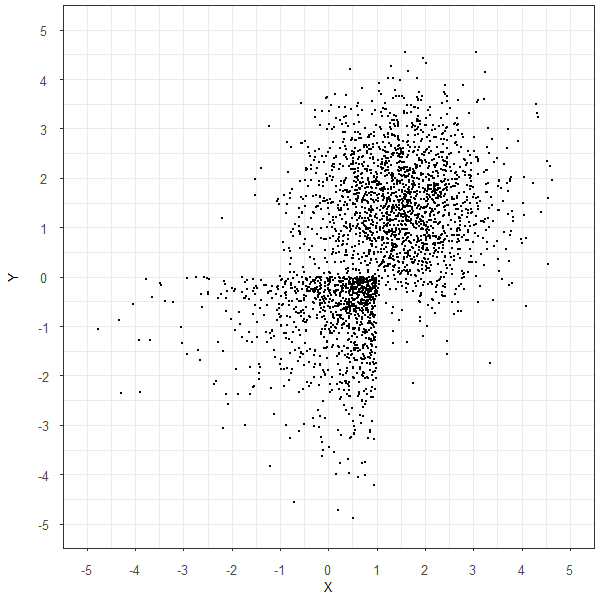
\includegraphics[scale=0.35]{6C__Users_tkpme_Dropbox_BookPCRA_Springer_Produ___hine_Learning_Plots_Scatter_plot_of_x_and_y.png}
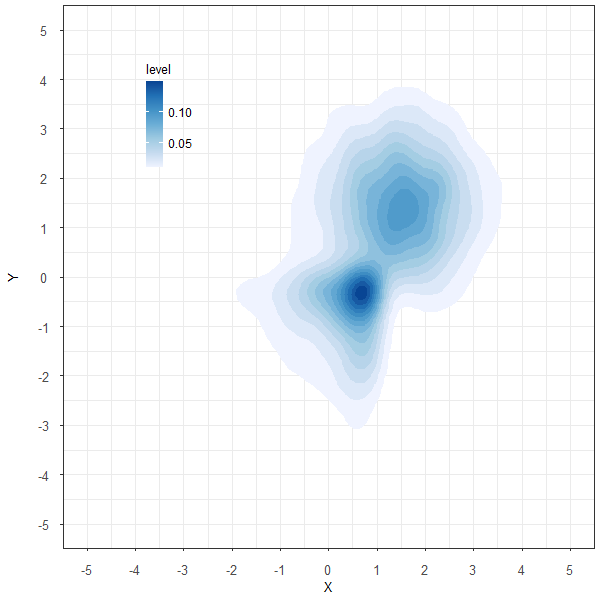
\includegraphics[scale=0.35]{7C__Users_tkpme_Dropbox_BookPCRA_Springer_Produ___nsity_plot_of_x_and_y_using_stat_density_2d.png}
\par\end{centering}
\begin{centering}
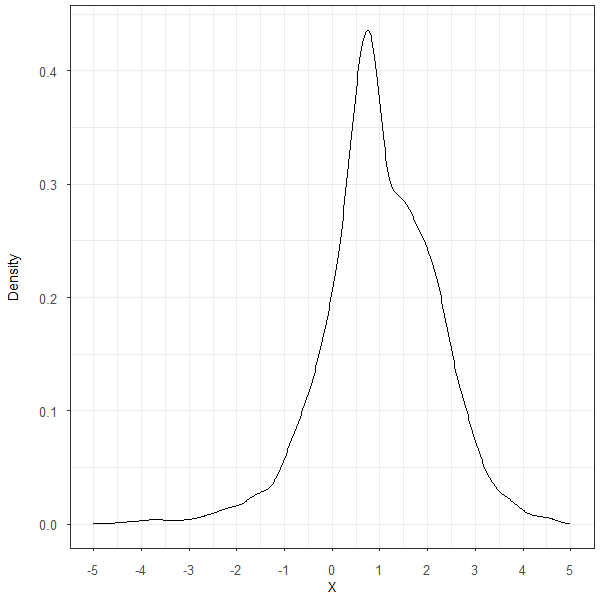
\includegraphics[scale=0.35]{8C__Users_tkpme_Dropbox_BookPCRA_Springer_Produ___hine_Learning_Plots_One-d_density_plot_of_x.png}
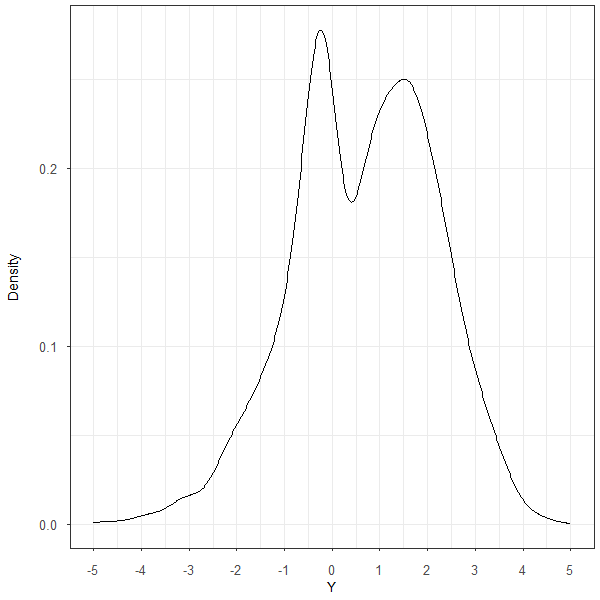
\includegraphics[scale=0.35]{9C__Users_tkpme_Dropbox_BookPCRA_Springer_Produ___hine_Learning_Plots_One-d_density_plot_of_y.png}
\par\end{centering}
\caption{\label{fig:Projections}Four views of two variables and their densities}
\end{figure}

Projection pursuit\footnote{The catchy name appears to have been first mentioned in \citet{FriedmanTukey1974}.}
is the process of exposing structure in a feature matrix beyond its
covariance matrix by maximizing an appropriately chosen \emph{projection
index $I$.} The value of the projection index ought to reflect how
interesting a particular projection of the features might be to an
analyst. The notion of interestingness is application dependent, but
is often interpreted as how non-normal the distribution of the projected
data is.

One-dimensional projection pursuit searches for a vector $\bubeta_{1}$
that best exposes the underlying structure of $\mathbf{X}$ by maximizing
$I\left(\mathbf{X}^{\prime}\,\bubeta\right)$. Two-dimensional projection
pursuit adds a second projection vector $\bubeta_{2}$ as well as
a bivariate projection index $I\left(\mathbf{X}^{\prime}\,\bubeta_{1},\ \mathbf{X}^{\prime}\,\bubeta_{2}\right)$
that is maximized when interesting structure in the joint density
of $\mathbf{X}$ in two orthogonal directions is best exposed.

Projection pursuit is often used to maximally separate clusters in
a feature matrix $\mathbf{X}$, and so lends itself to both supervised
and unsupervised learning. Projection pursuit regression goes a step
further -- it applies nonlinear transformations to projections of
data on a collection of identified proejction vectors to obtain a
better regression surface.

The R packages \texttt{Pursuit, tourr} and \texttt{REPPlab} allow
one to explore and visualize various projections of a data set, and
Figure \ref{fig:Iris1} displays two projections of the famous \texttt{iris}
dataset along two axes using \texttt{Pursuit::GrandTour}.\footnote{See \url{https://en.wikipedia.org/wiki/Iris_flower_data_set} for
the history of this dataset, which is widely used in machine learning.
It contains 4 measurements (the length and the width of petals and
sepals) on 150 flowers representing three species of irises. The measurements
were made by Edgar Anderson and the data set was made famous by Sir
Ronald Fisher in \citet{Fisher1936}.} The plot on the left displays the raw data projected without any
attempt to maximize separation between classes, and evidences significant
overlap between the three species. The plot on the right, in contrast,
shows how an optimal projection allows error-free identification of
all irises of species setosa, and excellent, though not perfect, separation
of the two other species (versicolor and virginica.)

\begin{figure}[H]
\begin{centering}
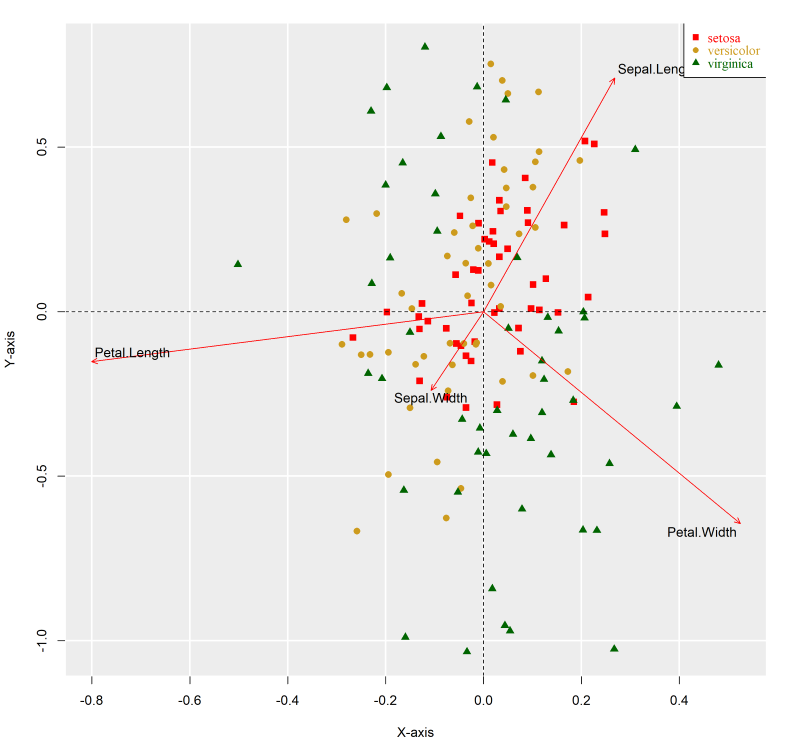
\includegraphics[width=7cm]{10C__Users_tkpme_Dropbox_BookPCRA_Springer_Prod___Learning_Plots_Projection_Pursuit_Unrotated.png}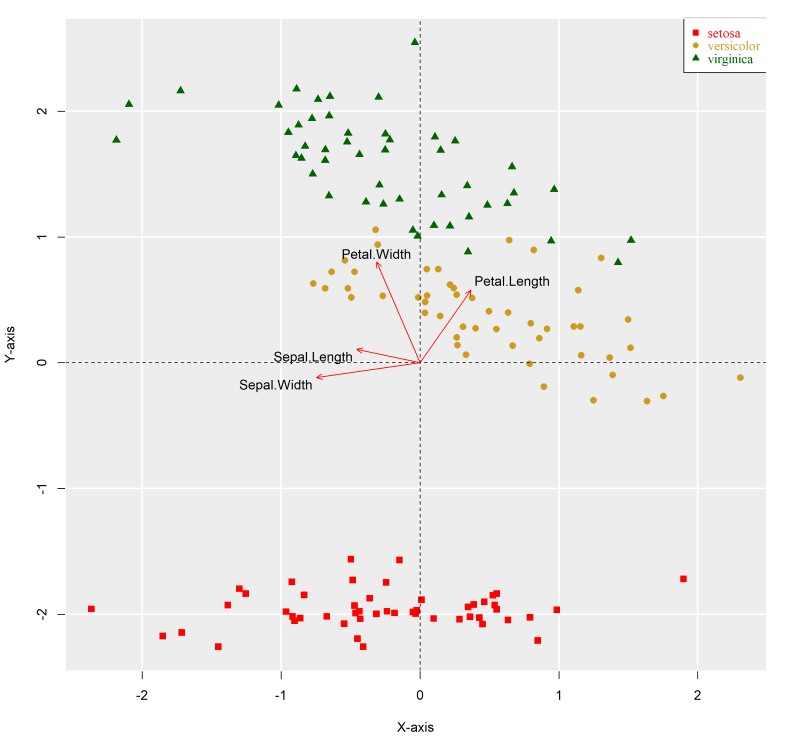
\includegraphics[width=7cm]{11C__Users_tkpme_Dropbox_BookPCRA_Springer_Prod___e_Learning_Plots_Projection_Pursuit_Example.png}
\par\end{centering}
\caption{\label{fig:Iris1}Initial and final projections of the Iris dataset}
\end{figure}

The projection vectors employed for the right-hand plot are displayed
in Table \ref{tab:ProjectionVectorsIris}, and it is easily confirmed
that they are orthogonal and have unit length. Projection pursuit
can be performed recursively -- all irises of class setosa can be
removed from the dataset, and the algorithm can then be applied to
separate irises of the two the remaining classes (versicolor and virginica)
as well as possible.

\begin{table}[H]
\caption{\label{tab:ProjectionVectorsIris}Unit projection vectors for Figure
\ref{fig:Iris1}}

\centering{}%
\begin{tabular}{ccc}
\toprule 
 &
\hphantom{22}Projection Vector 1 (X-axis)\hphantom{22} &
\hphantom{22}Projection Vector 2 (Y-axis)\hphantom{22}\tabularnewline
\midrule
\midrule 
Sepal.Length &
-0.4567710 &
0.1068818\tabularnewline
\midrule 
Sepal.Width &
-0.7476539 &
-0.1170979\tabularnewline
\midrule 
Petal.Length &
0.3671295 &
0.5765450\tabularnewline
\midrule 
Petal.Width &
-0.3123937 &
0.8015362\tabularnewline
\bottomrule
\end{tabular}
\end{table}

\citet{Kruskal1969} initiated work on projection pursuit by searching
for clusters that maximize an ``index of condensation'' which he
defined to be the coefficient of variation of the inter-point distances
generated by $\mathbf{X}\bubeta$, i.e.

\begin{equation}
I_{Kruskal}=\frac{\sigma_{y_{i}-y_{j}}}{\overline{y_{i}-y_{j}}}.\label{eq:KruskalCondensation}
\end{equation}

The intuition that motivates \eqref{eq:KruskalCondensation} is simple:
if projecting $\mathbf{X}$ onto $\bubeta$ results in a few well-separated
clusters of points, the average inter-point distance within clusters
will be small, while the average inter-point distance across clusters
will be large, simultaneously increasing its numerator and decreasing
its denominator. Unfortunately $I_{Kruskal}$ is not robust to outliers,
though it can be improved using robust estimates of both the numerator
and denominator.

Over the years, many such indices have been identified, and \citet{HouWentzell2011}
use kurtosis as an index to identify the directions $\mathbf{u}_{i}$
that maximize cluster separation by \emph{minimizing} the kurtosis
of $\mathbf{u}_{i}\cdot\mathbf{y}$. Their technique rests on \citet{Moors1986}
observation that kurtosis measures the dispersion of $x$ around both
$\mu-\sigma$ and $\mu+\sigma$, making its minimization a simple
way by which to optimally separate observations into two classes,
one centered at $\mu-\sigma$ and the other at $\mu+\sigma$. 

\begin{align}
\kappa & =E\left[\left(\frac{x\ -\ \mu}{\sigma}\right)^{4}\right]\nonumber \\
 & =E\left[\left(\left(\frac{x\ -\ \mu}{\sigma}\right)^{2}\right)^{2}\right]\nonumber \\
 & =E\left[\left(\left(\frac{x\ -\ \mu}{\sigma}\right)^{2}\right)\right]^{2}\ +\ \mathrm{var}\left(\left(\frac{x\ -\ \mu}{\sigma}\right)^{2}\right)\nonumber \\
 & =1\ +\ \mathrm{var}\left(\left(\frac{x\ -\ \mu}{\sigma}\right)^{2}\right)\label{eq:KurtosisForICA}
\end{align}

Figure \ref{fig:KurtosisMinProjections} and Table \ref{tab:KurtosisMinProjectionVector}
illustrates how the Iris dataset can be projected onto a single vector
and separated by minimizing kurtosis using the function \texttt{Pursuit::PP\_Optimizer}.
The results are virtually identical to those in Figure \ref{fig:Iris1}. 

\begin{figure}[H]
\begin{centering}
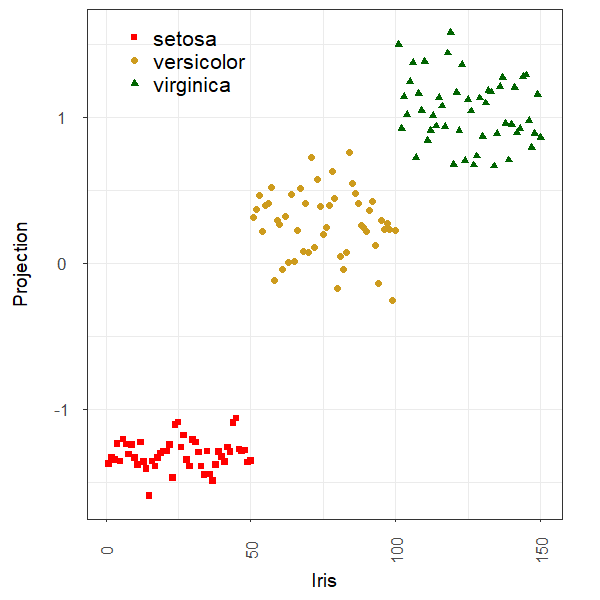
\includegraphics[width=10cm]{12C__Users_tkpme_Dropbox_BookPCRA_Springer_Prod___achine_Learning_Plots_Kurtosis_Minimization.png}
\par\end{centering}
\caption{\label{fig:KurtosisMinProjections}Projections onto the kurtosis minimizing
projection vector}
\end{figure}

\begin{table}[H]
\caption{\label{tab:KurtosisMinProjectionVector}The kurtosis minimizing projection
vector}

\centering{}%
\begin{tabular}{cc}
\toprule 
Feature &
\hphantom{22222} Projection Vector\tabularnewline
\midrule
\midrule 
Sepal.Length &
0.988068380 \hphantom{22}\tabularnewline
\midrule 
Sepal.Width &
0.114840009 \hphantom{22}\tabularnewline
\midrule 
Petal.Length &
-0.102380058 \hphantom{22}\tabularnewline
\midrule 
Petal.Width &
0.007139457 \hphantom{22}\tabularnewline
\bottomrule
\end{tabular}
\end{table}

Projection pursuit analysis (PPA) has much in common with Independent
Components Analysis (ICA), which in turn is related to Principal Components
Analysis (PCA). The links between the techniques are addressed briefly
in Chapter 14 of \citet{HastieTibshiraniFriedman2009} and are developed
comprehensively in \citet{HyvarinenOja2000} and \citet{HyvarinenKaarhunenOja2001}. 

\subsection{Projection Pursuit Regression}

\citet{FriedmanStuetzle1981} use the projections identified by PPA
to usefully generalize Least Squares\footnote{See \ProbabilityAppendix\ for a development of Least Squares.}
by writing 

\begin{equation}
\hat{y}=\overline{y}\ +\ \sum_{i=1}^{m}f_{i}\left(\mathbf{x}^{\prime}\,\bubeta_{i}\right),\label{eq:PPR1}
\end{equation}

where $\bubeta_{i}$ is the $i^{th}$ projection,\footnote{These may not be identical to the projections identified by projection
pursuit.} and $f_{i},\ 1\leqslant i\leqslant m$ are smooth \emph{ridge functions},
or functions that vary only in the direction of $\bubeta$.\footnote{See \citet{KonyaginKuleshovMaiorov2018} for the theory of ridge functions.}
The ridge functions in \eqref{eq:PPR1}are not restricted to be linear,
allowing it to capture nonlinearities in the relationship between
$\mathbf{x}$ and $y$. Most importantly, \citet{DiaconisShahshahani1984}
show that ridge functions possess a universal approximation property
-- any function of $p$ variables can be appproximated arbitrarily
well by ridge functions for sufficiently large $m$, echoing the Stone-Weierstrass
Theorem for continuous functions on Hausdorff spaces.

\citet{FriedmanStuetzle1981} call their method Projection Pursuit
Regression (PPR) and present an iterative algorithm for identifying
$m$, $f_{i}$ and $\bubeta_{i}$. Even though the algorithm is refined
in \citet{Friedman1985} and \citet{Friedman1987}, we present only
the original version, both for ease of exposition and for relevance.
In spite of its distinguished parentage, PPR is no longer widely used,
and lives on primarily as the intellectual predecessor of neural networks,
largely on account of the universal approximation property they share.

\begin{algorithm}[H]
\begin{enumerate}
\item \texttt{Initialize:}
\begin{enumerate}
\item $i\longleftarrow1$
\item $m\longleftarrow m_{max}$
\item \texttt{Demean the response vector} $\mathbf{y}_{1}\longleftarrow\mathbf{y}-\bar{\mathbf{y}}\mathbf{1}$\medskip{}
\end{enumerate}
\item \texttt{While $i=1,\ 2,\cdots,\ m$ and ($res^{2}$> Threshold):}
\begin{enumerate}
\item \texttt{Compute the residuals $\mathrm{\bueps}_{i}\longleftarrow\mathbf{y}_{i}\ -\ \sum_{j=1}^{i-1}f_{j}\left(\mathbf{X}\,\bubeta_{j}\right)$}
\item \texttt{Search for and dentify the $i^{th}$ projection vector }$\bubeta_{i}$
\texttt{and ridge function} $f_{i}$ \texttt{that minimizes the sum
of squared residuals} $res^{2}=\left(\mathrm{\bueps}_{i}\ -\ f_{i}\left(\mathbf{X}\,\bubeta_{i}\right)\right)^{\prime}\left(\mathrm{\bueps}_{i}\ -\ f_{i}\left(\mathbf{X}\,\bubeta_{i}\right)\right)$
, where $f_{i}\left(\cdot\right)$is applied to each component of
$\mathbf{X}\,\bubeta_{i}$.\bigskip{}
\end{enumerate}
\end{enumerate}
\caption{\label{alg:FriedmanSteutzlePPR}The Friedman-Steutzle algorithm for
Projection Pursuit Regression}
\end{algorithm}

Algorithm \ref{alg:FriedmanSteutzlePPR} is a forward stagewise procedure
-- once a projection vector is identified, it is not modified in
later stages. In contrast, the SMART algorithm decribed in \citet{Friedman1985}
directly minimizes the sum of squared residuals by iteratively minimizing
the magnitude of the residual \eqref{eq:PPR1} using a Gauss-Newton
iteration

\begin{equation}
m^{*},\ \mathbf{f}^{*},\ \bubeta^{*}=\underset{m,\ f_{i},\ \bubeta_{i}}{argmin}\left(\mathbf{y}\ -\ \bar{\mathbf{y}}\mathbf{1}\ -\ \sum_{i=1}^{m}f_{i}\left(\mathbf{X}\,\bubeta_{i}\right)\right)^{\prime}\left(\mathbf{y}\ -\ \bar{\mathbf{y}}\mathbf{1}\ -\ \sum_{i=1}^{m}f_{i}\left(\mathbf{X}\,\bubeta_{i}\right)\right),\label{eq:SMARTppr}
\end{equation}

where $m^{*},\ \mathbf{f}^{*}$ and $\bubeta^{*}$ are the optimal
values of $m$, $f_{i},\ 1\leqslant i\leqslant m$ and $\bubeta_{i},\ 1\leqslant i\leqslant m$. 

The two solutions can be strikingly different, particularly when the
features are almost collinear. The SMART algorithm is available as
the Base R functions \texttt{ppr} and \texttt{plot.ppr}. 

Table \ref{tab:pprFitofFNBtoF3andFFC4} displays the projection vectors
identified by PPR as well as the LS fits of Fama-French 3-- and 4--factor
models to the weekly returns of the stock with ticker FNB in 2008.
It echoes the comparison between LS and robust regression in \FNBLSandRobustRegressionTable.
We have deliberately suppressed the intercept as it is small, and
as the projection vectors do not have an intercept. The first four
columns display the first two projection vectors for PPR for the 3--
and 4--factor Fama-French models while the last two columns display
LS fits using the same data. It is not possible to display or compactly
characterize the entire PPR surface as it involves non-linear smoothing
of the residuals generated by each of the ridge functions.

\begin{table}[H]
\caption{\label{tab:pprFitofFNBtoF3andFFC4}Projection Pursuit Vectors and
LS fits of FF3 and FFC4 models to FNB 2008 weekly returns.}

\begin{kframe}


{\ttfamily\noindent\bfseries\color{errorcolor}{\#\# Error in `readChar()`:\\\#\# ! cannot open the connection}}

{\ttfamily\noindent\bfseries\color{errorcolor}{\#\# Error in `readChar()`:\\\#\# ! cannot open the connection}}

{\ttfamily\noindent\bfseries\color{errorcolor}{\#\# Error in `readChar()`:\\\#\# ! cannot open the connection}}

{\ttfamily\noindent\bfseries\color{errorcolor}{\#\# Error:\\\#\# ! object 'stkLs\_' not found}}

{\ttfamily\noindent\bfseries\color{errorcolor}{\#\# Error:\\\#\# ! object 'stkLs\_' not found}}

{\ttfamily\noindent\bfseries\color{errorcolor}{\#\# Error:\\\#\# ! object 'FNB' not found}}

{\ttfamily\noindent\bfseries\color{errorcolor}{\#\# Error:\\\#\# ! object 'FNB' not found}}

{\ttfamily\noindent\bfseries\color{errorcolor}{\#\# Error:\\\#\# ! object 'FNB' not found}}

{\ttfamily\noindent\bfseries\color{errorcolor}{\#\# Error:\\\#\# ! object 'FNB\_FF3' not found}}

{\ttfamily\noindent\bfseries\color{errorcolor}{\#\# Error:\\\#\# ! object 'FNB\_FF3' not found}}

{\ttfamily\noindent\bfseries\color{errorcolor}{\#\# Error:\\\#\# ! object 'FNB\_FF4' not found}}

{\ttfamily\noindent\bfseries\color{errorcolor}{\#\# Error:\\\#\# ! object 'FNB\_FF4' not found}}

{\ttfamily\noindent\bfseries\color{errorcolor}{\#\# Error:\\\#\# ! object 'FNB\_FF3.ppr' not found}}

{\ttfamily\noindent\bfseries\color{errorcolor}{\#\# Error:\\\#\# ! object 'FNB\_FF3.alpha' not found}}

{\ttfamily\noindent\bfseries\color{errorcolor}{\#\# Error:\\\#\# ! object 'FNB\_FF4.ppr' not found}}

{\ttfamily\noindent\bfseries\color{errorcolor}{\#\# Error:\\\#\# ! object 'FNB\_FF4.alpha' not found}}

{\ttfamily\noindent\bfseries\color{errorcolor}{\#\# Error:\\\#\# ! object 'FNB\_FF3.lm' not found}}

{\ttfamily\noindent\bfseries\color{errorcolor}{\#\# Error:\\\#\# ! object 'lsFBB\_FF3.coef' not found}}

{\ttfamily\noindent\bfseries\color{errorcolor}{\#\# Error:\\\#\# ! object 'FNB\_FF4.lm' not found}}

{\ttfamily\noindent\bfseries\color{errorcolor}{\#\# Error:\\\#\# ! object 'lsFBB\_FF4.coef' not found}}

{\ttfamily\noindent\bfseries\color{errorcolor}{\#\# Error:\\\#\# ! object 'FNB\_FF3.alpha' not found}}

{\ttfamily\noindent\bfseries\color{errorcolor}{\#\# Error:\\\#\# ! object 'projVectorsAndCoeffs' not found}}

{\ttfamily\noindent\bfseries\color{errorcolor}{\#\# Error in `column\_spec()`:\\\#\# ! could not find function "{}column\_spec"{}}}\end{kframe}
\end{table}

Table \ref{tab:rssFNBtoF3andFFC4} displays the residual sums of squares
for PPR and LS fits to the weekly returns of FNB in 2008. PPR roughly
halves the error variance, in part due to the fact that it fits the
data with non-linear ridge functions. It is striking that both fits
see little improvement when moving from three factors to four, supporting
the widely-held view that equity returns are explained in large part
by a few systematic factors.

\begin{table}[H]
\caption{\label{tab:rssFNBtoF3andFFC4}Residual Sum of Squares for PPR and
LS fits of FF3 and FFC4 models to FNB 2008 weekly returns.}

\begin{kframe}


{\ttfamily\noindent\bfseries\color{errorcolor}{\#\# Error:\\\#\# ! object 'FNB\_FF3.ppr' not found}}

{\ttfamily\noindent\bfseries\color{errorcolor}{\#\# Error:\\\#\# ! object 'FNB\_FF4.ppr' not found}}

{\ttfamily\noindent\bfseries\color{errorcolor}{\#\# Error:\\\#\# ! object 'FNB\_FF3.lm' not found}}

{\ttfamily\noindent\bfseries\color{errorcolor}{\#\# Error:\\\#\# ! object 'FNB\_FF4.lm' not found}}

{\ttfamily\noindent\bfseries\color{errorcolor}{\#\# Error:\\\#\# ! object 'rss.FNB\_FF3.ppr' not found}}

{\ttfamily\noindent\bfseries\color{errorcolor}{\#\# Error in `colnames<-`:\\\#\# ! attempt to set 'colnames' on an object with less than two dimensions}}

{\ttfamily\noindent\bfseries\color{errorcolor}{\#\# Error in `column\_spec()`:\\\#\# ! could not find function "{}column\_spec"{}}}\end{kframe}
\end{table}

\end{appendices}

\pagebreak{}

\begin{flushleft}
\printbibliography
\par\end{flushleft}

\newpage
\end{document}
